% RepNet Progress Update — Finalized Model Performance
% Same visual identity as final_presentation_modern.tex
% Compiles with pdfLaTeX.

\documentclass[10pt,aspectratio=169]{beamer}

% ====================
% Packages
% ====================
\usepackage[T1]{fontenc}
\usepackage{lmodern}
\usepackage{graphicx}
\usepackage{booktabs}
\usepackage{mathtools}
\usepackage{tikz}
\usetikzlibrary{positioning,arrows.meta}
\usepackage{hyperref}
\usepackage{pgfplots}
\pgfplotsset{compat=1.18}

% ====================
% UC Davis brand colors (digital palette)
% ====================
\definecolor{aggieblue}{HTML}{022851}
\definecolor{aggiegold}{HTML}{FFBF00}
\definecolor{aggieblueDark}{HTML}{011936}
\definecolor{aggiegoldDark}{HTML}{C99700}
\definecolor{coolgray}{RGB}{77,79,83}
\definecolor{boxgray}{RGB}{238,235,233}

% ====================
% Fonts
% ====================
\renewcommand{\familydefault}{\sfdefault}
\newcommand{\Raleway}{\sffamily}
\newcommand{\Lato}{\sffamily}

% ====================
% Beamer color slots
% ====================
\setbeamercolor*{palette primary}{fg=white,bg=aggieblue}
\setbeamercolor*{palette secondary}{fg=white,bg=coolgray}
\setbeamercolor*{palette tertiary}{fg=white,bg=aggieblueDark}
\setbeamercolor*{palette quaternary}{fg=aggieblue,bg=aggiegold}

\setbeamercolor{structure}{fg=aggieblue}
\setbeamercolor{titlelike}{fg=aggieblue}
\setbeamercolor{frametitle}{fg=white,bg=aggieblue}
\setbeamercolor{title}{fg=white,bg=aggieblue}
\setbeamercolor{author}{fg=aggieblue}
\setbeamercolor{institute}{fg=coolgray}
\setbeamercolor{date}{fg=coolgray}

\setbeamercolor{section in toc}{fg=aggieblue}
\setbeamercolor{subsection in toc}{fg=aggieblueDark}

% ====================
% Fonts (sizes/weights)
% ====================
\setbeamerfont{title}{family=\Raleway,series=\bfseries,size=\LARGE}
\setbeamerfont{subtitle}{family=\Lato,size=\normalsize}
\setbeamerfont{author}{family=\Lato,size=\small}
\setbeamerfont{institute}{family=\Lato,size=\footnotesize}
\setbeamerfont{date}{family=\Lato,size=\footnotesize}
\setbeamerfont{frametitle}{family=\Raleway,series=\bfseries,size=\large}
\setbeamerfont{section in toc}{family=\Raleway,series=\bfseries}
\setbeamerfont{subsection in toc}{family=\Lato,size=\small}
\setbeamerfont{footline}{family=\Lato,size=\scriptsize}

% ====================
% Frame title with Aggie Gold accent bar
% ====================
\setbeamertemplate{frametitle}{%
  \nointerlineskip
  \begin{beamercolorbox}[wd=\paperwidth,ht=3.0ex,dp=1.4ex,leftskip=1em,rightskip=1em]{frametitle}%
    \usebeamerfont{frametitle}\insertframetitle%
  \end{beamercolorbox}%
  \begin{beamercolorbox}[wd=\paperwidth,ht=0.35ex,dp=0pt]{palette quaternary}%
  \end{beamercolorbox}%
  \vspace{1.0ex}
}

\beamertemplatenavigationsymbolsempty

% ====================
% Table of Contents Customization
% ====================
\setbeamertemplate{section in toc}{\leavevmode\inserttocsection\par}

\setbeamertemplate{subsection in toc}{%
  \leavevmode\hspace{1.5em}%
  \color{aggiegoldDark}\raise0.4ex\hbox{\vrule width 0.4ex height 0.4ex}%
  \hspace{0.5em}\color{aggieblueDark}\inserttocsubsection\par
}

% ====================
% Footer
% ====================
\newcommand{\footercontent}[1]{\renewcommand{\insertfootercontent}{#1}}
\newcommand{\insertfootercontent}{}

\setbeamertemplate{footline}{%
  \ifx\insertfootercontent\@empty\else
    \begin{beamercolorbox}[wd=\paperwidth,ht=0.3ex,dp=0pt]{palette quaternary}\end{beamercolorbox}%
    \begin{beamercolorbox}[wd=\paperwidth,ht=2.4ex,dp=1.2ex,leftskip=1em,rightskip=1em]{palette primary}%
      \usebeamerfont{footline}\insertfootercontent\hfill\insertframenumber{}/\inserttotalframenumber%
    \end{beamercolorbox}%
  \fi
}

% ====================
% Title / authors
% ====================
\title{Risk Estimation of Preeclampsia}
\subtitle{}
\author{Ahmed Khan \and Lawrencedel Legaspi \and Selena Phu}
\institute{Department of Electrical and Computer Engineering \\ University of California, Davis}
\date{\today}

\titlegraphic{}

\footercontent{%
  \href{https://github.com/AhmedKhan-GH/repnet}{github.com/AhmedKhan-GH/repnet}
  \enspace$\bullet$\enspace
  UC Davis Senior Design 2026%
}

% ====================
% Title page template
% ====================
\setbeamertemplate{title page}{%
  \begin{tikzpicture}[remember picture,overlay]
    \fill[aggieblue]
      ([yshift=1cm]current page.north west)
      rectangle
      ([yshift=-3.8cm]current page.north east);
    \fill[aggiegold]
      ([yshift=-3.8cm]current page.north west)
      rectangle
      ([yshift=-3.95cm]current page.north east);
    \node[anchor=center,text=white,align=center,text width=10cm,
          font=\Raleway\bfseries]
      at ([yshift=-2.2cm]current page.north)
      {\usebeamerfont{title}\inserttitle};
    \node[anchor=center,text=aggiegold,align=center,text width=14cm,
          font=\Lato]
      at ([yshift=-2.4cm]current page.north)
      {\usebeamerfont{subtitle}\insertsubtitle};
    \node[anchor=north,text=aggieblue,align=center,font=\Lato]
      at ([yshift=-5.4cm]current page.north)
      {\usebeamerfont{author}\insertauthor};
    \node[anchor=north,text=coolgray,align=center,font=\Lato]
      at ([yshift=-6.0cm]current page.north)
      {\usebeamerfont{institute}\insertinstitute};
    \node[anchor=north,text=coolgray,align=center,font=\Lato]
      at ([yshift=-6.9cm]current page.north)
      {\usebeamerfont{date}\insertdate};
  \end{tikzpicture}%
}

% ====================
% 3D block drawing helper (x, y, width, height, depth, color)
% ====================
\newcommand{\tblock}[6]{%
  \pgfmathsetmacro{\tbw}{#3}\pgfmathsetmacro{\tbh}{#4}%
  \pgfmathsetmacro{\tbdx}{0.15*#5}\pgfmathsetmacro{\tbdy}{0.15*#5}%
  \fill[#6, opacity=0.8] (#1,#2) rectangle ++(#3,#4);
  \draw[#6!40!black] (#1,#2) rectangle ++(#3,#4);
  \fill[#6!75!white, opacity=0.6]
    (#1,{#2+#4}) -- ++(\tbdx,\tbdy) -- ++(#3,0) -- ++({-\tbdx},{-\tbdy}) -- cycle;
  \draw[#6!40!black]
    (#1,{#2+#4}) -- ++(\tbdx,\tbdy) -- ++(#3,0) -- ++({-\tbdx},{-\tbdy}) -- cycle;
  \fill[#6!55!black, opacity=0.5]
    ({#1+#3},#2) -- ++(\tbdx,\tbdy) -- ++(0,#4) -- ++({-\tbdx},{-\tbdy}) -- cycle;
  \draw[#6!40!black]
    ({#1+#3},#2) -- ++(\tbdx,\tbdy) -- ++(0,#4) -- ++({-\tbdx},{-\tbdy}) -- cycle;
}

% ====================
% Hidden section declarations to populate the TOC
% ====================
\section{Introduction}
\section{Decision-Tree Modeling}
\subsection{Dataset Profile}
\subsection{Feature Extraction}
\subsection{Feature Importance}
\subsection{Feature Selection Matrix}
\subsection{Individual vs.\ Ensemble Performance}
\section{Neural Network Modeling}
\subsection{Preprocessing \& Training}
\subsection{Depthwise Separable Convolution}
\subsection{Squeeze-Excitation}
\subsection{Multi-Head Cross-Lead Attention}
\subsection{Model Performance}
\subsection{Interpretability}
\section{Conclusion}
\section{Future Work}


% ====================
% Document
% ====================
\begin{document}

% ---------- Title Slide ----------
{%
  \setbeamertemplate{footline}{}%
  \begin{frame}[plain,noframenumbering]
    \titlepage
  \end{frame}
}

% ---------- Table of Contents Slide ----------
\begin{frame}{Contents}
  \tableofcontents
\end{frame}

% ---------- Preeclampsia Introduction Slide ----------

\begin{frame}{Preeclampsia Introduction}
  \begin{columns}[T]

    % --- Left Column: Definition, Goal, Infographic, and Clinical ECG Setup ---
    \begin{column}{0.52\textwidth}
      \usebeamerfont{footline}\color{coolgray}
      
      % Main Bullets
      \begin{itemize}
        \item Cannot be cured until birth
        \item Can progress to severe at a quick rate
        \item Leading cause of maternal and infant illness and death
      \end{itemize}

      \vspace{0.5em}

      % Blue Goal Highlight Box
      \setbeamercolor{boxblue}{bg=aggieblue,fg=white}
      \begin{beamercolorbox}[wd=\textwidth,rounded=true,leftskip=0.7em,rightskip=0.7em,sep=0.6em]{boxblue}
        \scriptsize\Lato\bfseries\color{white}
        Current goal: predict the risk of Preeclampsia using Decision Tree Modeling and Neural Network Modeling
      \end{beamercolorbox}

      \vspace{0.8em}

      % Side-by-Side Images at the bottom of the left column
      \begin{minipage}[t]{0.48\textwidth}
        \centering
        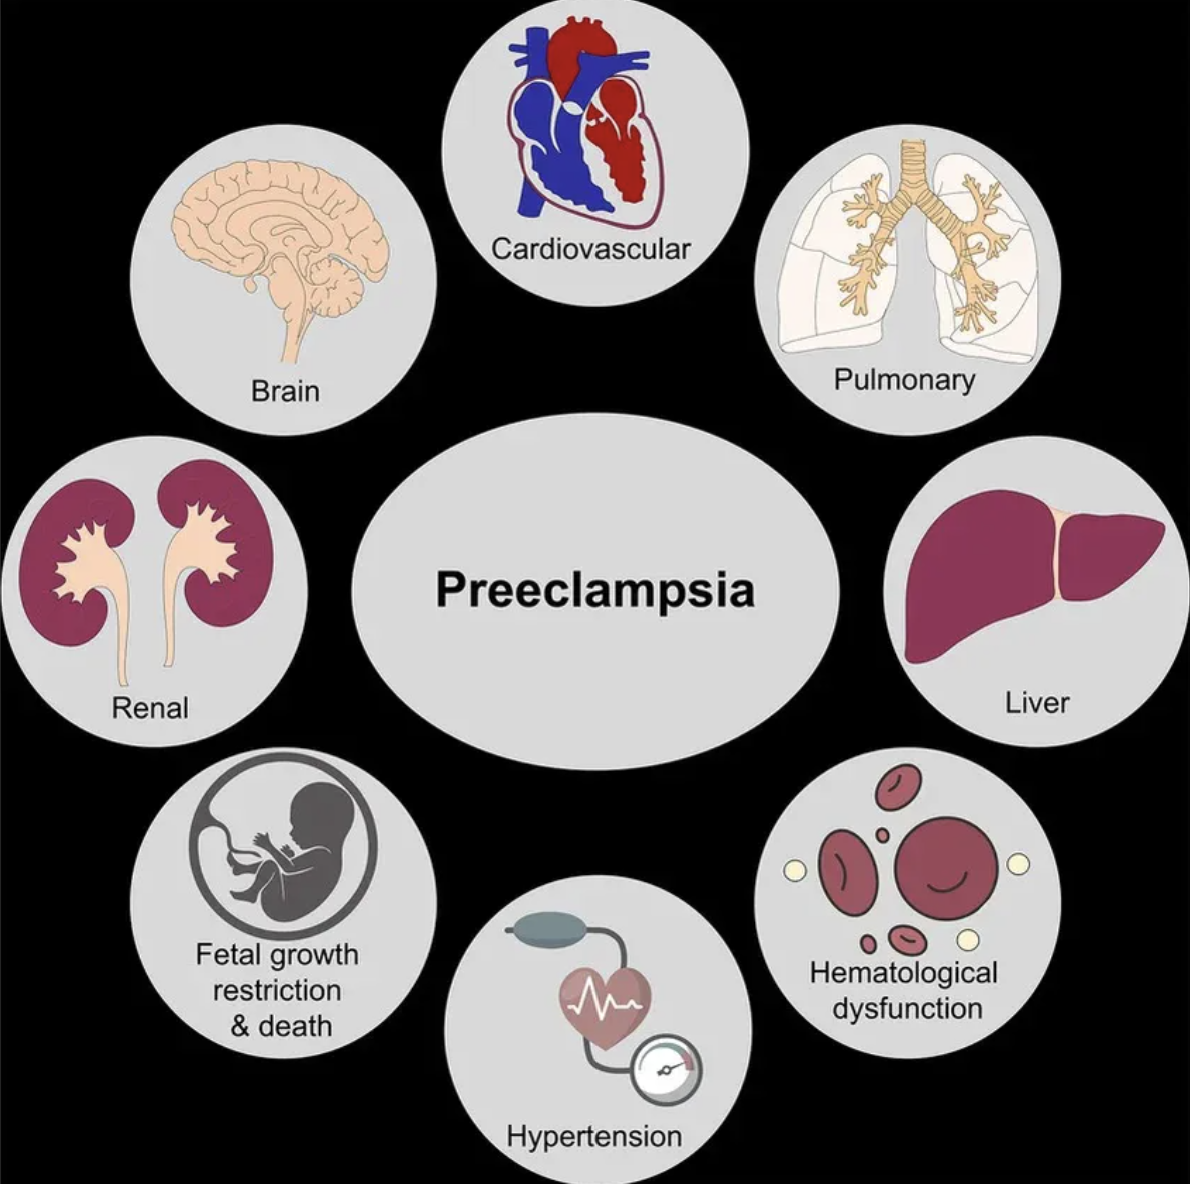
\includegraphics[width=\textwidth]{preeclampsia_infographic.png}
      \end{minipage}
      \hfill
      \begin{minipage}[t]{0.48\textwidth}
        \centering
        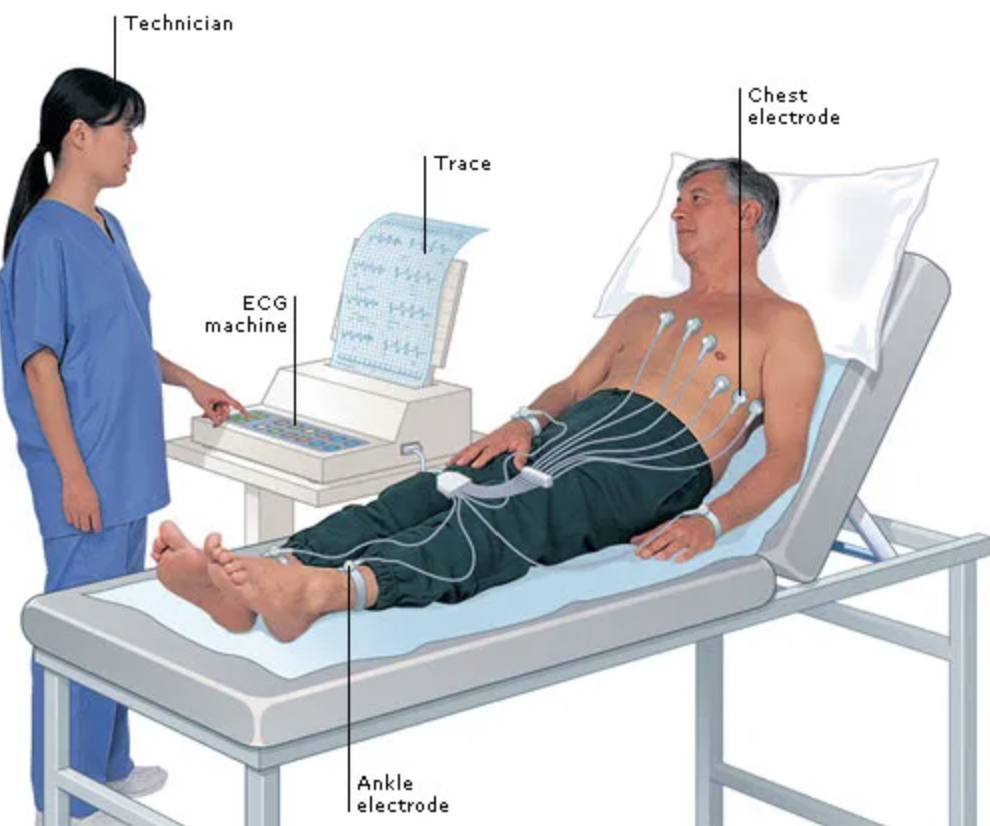
\includegraphics[width=\textwidth]{bed.png} % This is the medical setup diagram
      \end{minipage}
    \end{column}

    % --- Right Column: Electrode Positioning Diagrams Stacked with Headers ---
    \begin{column}{0.44\textwidth}
      \centering
      
      % Top Image: Precordial Leads
      \vspace{-1em}
      {\footnotesize\Raleway\color{aggieblue} Precordial Leads}\\[0.2em]
      \begin{center}
        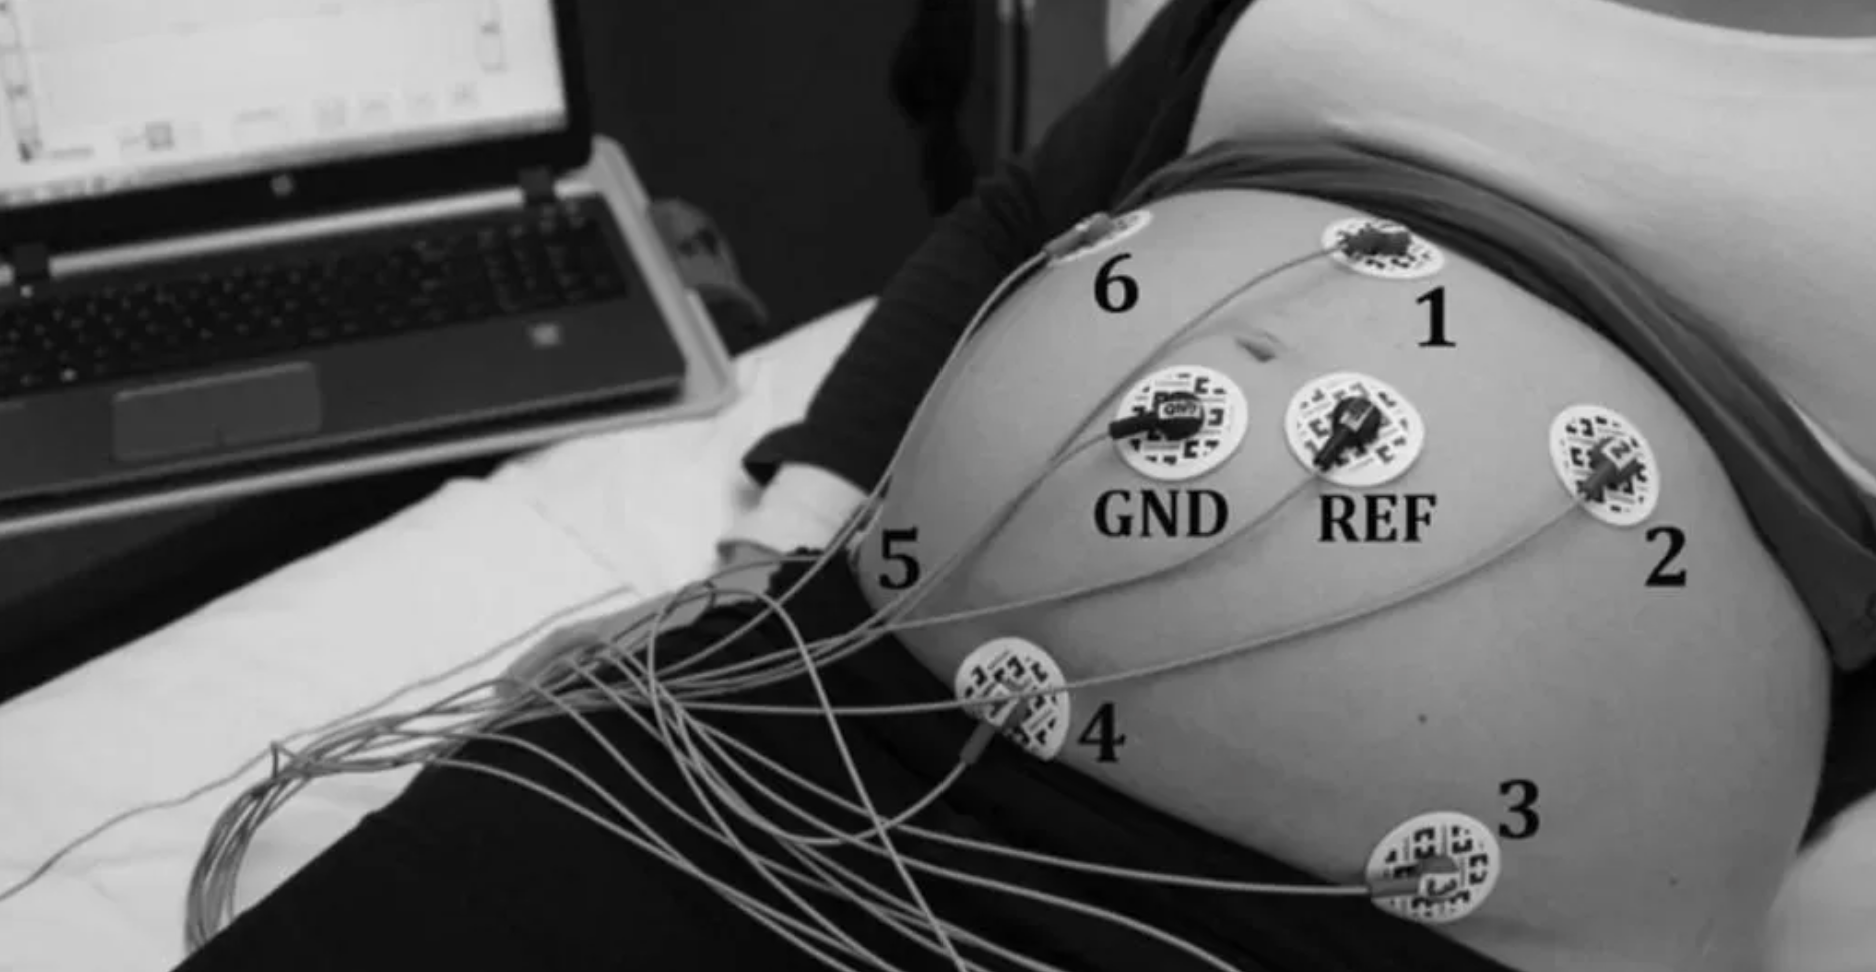
\includegraphics[width=0.80\textwidth]{pregnant.png}
      \end{center}

      \vspace{0.2em}

      % Bottom Image: Limb Leads
      {\footnotesize\Raleway\color{aggieblue} Limb Leads}\\[0.2em]
      \begin{center}
        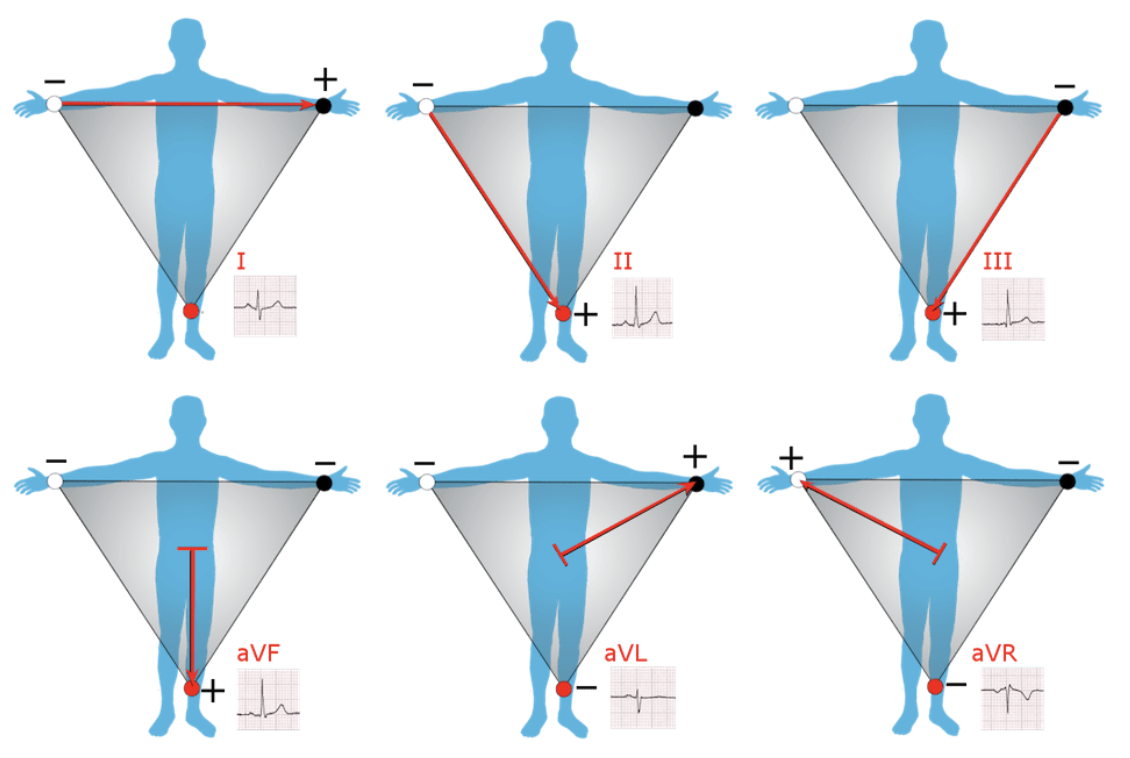
\includegraphics[width=0.75\textwidth]{limb_leads.png}
      \end{center}
    \end{column}

  \end{columns}
\end{frame}

% ---------- Transition Slide ----------
{%
  \setbeamertemplate{footline}{}%
  \begin{frame}[plain,noframenumbering]
    \begin{tikzpicture}[remember picture,overlay]
      \fill[aggieblue] (current page.south west) rectangle (current page.north east);
    \end{tikzpicture}
    \vfill
    \centering
    {\Raleway\bfseries\Huge\color{white} Decision-Tree Modeling}\\[0.6em]
    {\color{aggiegold}\rule{6cm}{0.06cm}}
    \vfill
  \end{frame}
}

% ---------- Subsection Slide: Dataset Profile ----------
\begin{frame}{Decision-Tree Modeling --- Dataset Profile}
  \begin{columns}[T]
    
    % Left Column: Reduced width to give signals more room
    \begin{column}{0.42\textwidth} 
      \centering
      {\small\Raleway\bfseries\color{aggieblue} ECG Dataset Breakdown}\\[1.5em]
      
      \renewcommand{\arraystretch}{1.8}
      \resizebox{\textwidth}{!}{%
        \begin{tabular}{lccc}
          \toprule
          \textbf{Dataset} & \textbf{\shortstack{Original Total\\(P/N)}} & \textbf{\shortstack{Dropped ECGs\\(P/N)}} & \textbf{\shortstack{Final Total\\(P/N)}} \\
          \midrule
          Unbalanced & 337 / 1854 & 8 / 24 & 329 / 1830 \\
          Balanced   & 187 / 182  & 6 / 1  & 181 / 181 \\
          \bottomrule
        \end{tabular}
      }
      \vspace{0.3em}
      \begin{flushleft}
      \usebeamerfont{footline}\color{coolgray}
       Each ECG sample includes \textbf{656 distinct MUSE metadata features}\\[0.8em]
      
      \textbf{Cross-Validation Strategy:}
      \begin{itemize}
        \item \textbf{StratifiedGroupKFold} with 5 folds grouped by the Patient's MRN
        \item \textbf{RandomForest} with \textbf{RandomUnderSampler} inside the folds
      \end{itemize}
      \end{flushleft}
    \end{column}
    
    % Right Column: Increased width (from 0.44 to 0.54)
    \begin{column}{0.54\textwidth}
      \centering
      {\small\Raleway\bfseries\color{aggieblue} Signal Preprocessing}\\[1.0em]
      
      \begin{beamercolorbox}[wd=\textwidth,rounded=true,shadow=false,sep=0.2em]{boxgray}
        \centering
        % Removed keepaspectratio to force the plot to fill the full column width
        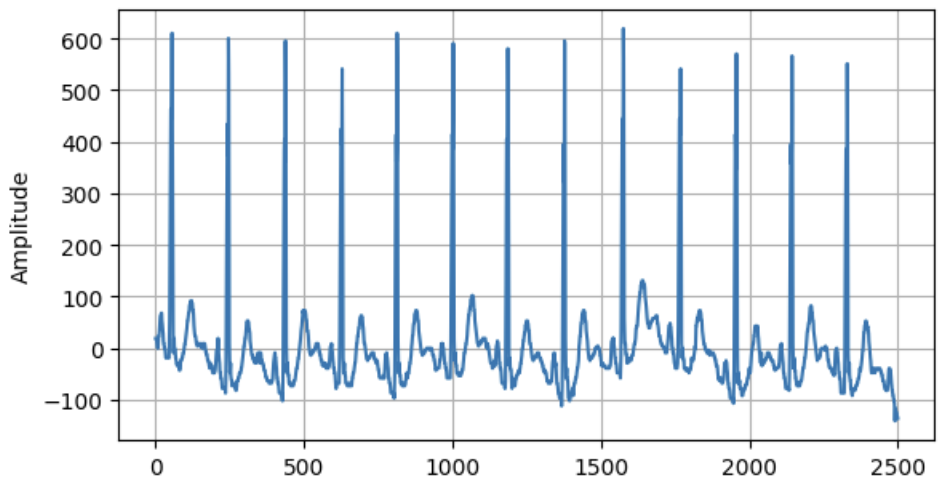
\includegraphics[width=1\textwidth,height=2.3cm]{v3_pre.png}
        
        \vspace{0.4em}
        
        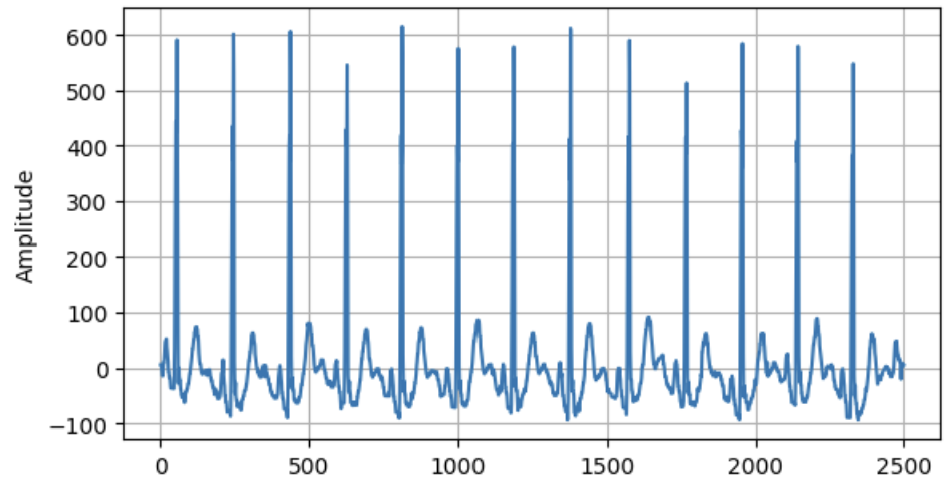
\includegraphics[width=1\textwidth,height=2.3cm]{v3_filter.png}
      \end{beamercolorbox}
    
    \end{column}

  \end{columns}
\end{frame}

% ---------- Subsection Slide: Feature Extraction ----------
% ---------- Subsection Slide: Feature Extraction ----------
\begin{frame}{Decision-Tree Modeling --- Feature Extraction}
  \begin{columns}[c] 
    
    % Left Column: Image
    \begin{column}{0.45\textwidth}
      \centering
      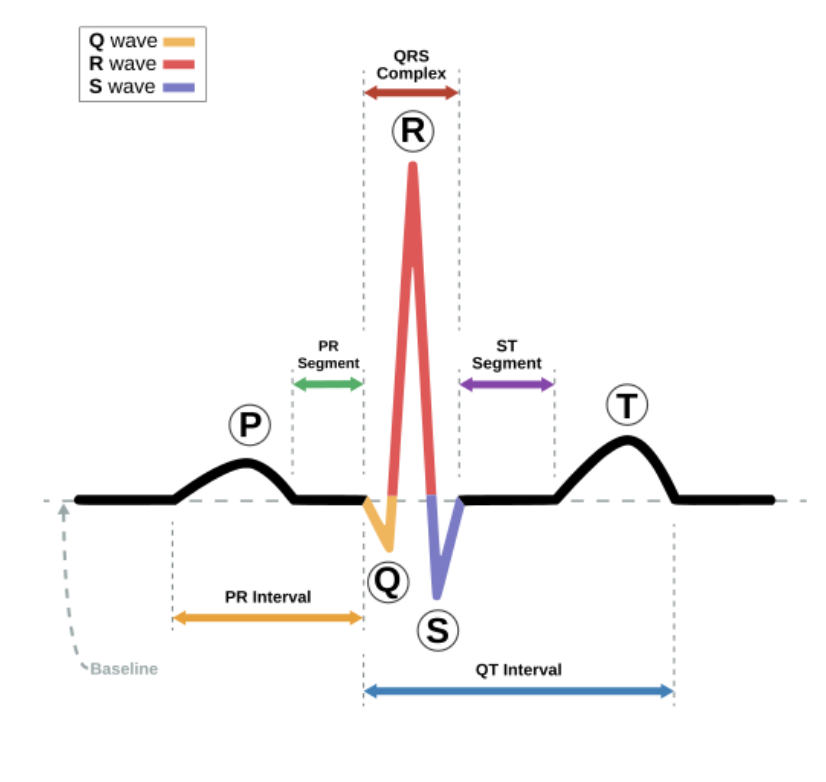
\includegraphics[width=\textwidth]{featurization.png}
    \end{column}
    
    % Right Column: Content pulled upward with larger font
    \begin{column}{0.50\textwidth}
      \vspace{-3.5em} % Adjusted slightly down to accommodate the larger text height
      
      \begin{large} % <--- Bumps the text size up to large
      \begin{itemize}
        \setlength{\itemsep}{1.2em} 
        
        \item \textbf{Feature Extraction:}
        \vspace{0.6em}
        \begin{itemize}
          \setlength{\itemsep}{0.6em} 
          \item \textbf{NeuroKit}
          \item \textbf{MUSE-derived} 
        \end{itemize}
        
      \end{itemize}
      \end{large}
      
    \end{column}

  \end{columns}
\end{frame}
% ---------- Subsection Slide: Model Performance ----------
\begin{frame}{Decision-Tree Modeling --- Feature Importance}
  \centering
  {\small\Raleway\bfseries\color{aggieblue} Random Forest Performance}\\[0.3em]
  
  \resizebox{0.95\textwidth}{!}{%
    \begin{tabular}{lcccccccc}
      \toprule
      \textbf{Method} & \textbf{\# Features} & \textbf{AUROC} & \textbf{AUPRC} & \textbf{Specificity} & \textbf{Sensitivity} & \textbf{Bal. Accuracy} & \textbf{Precision} & \textbf{F1-Score} \\
      \midrule
      Original & 723 & $69.93 \pm 3.30$ & $32.55 \pm 3.71$ & $73.74 \pm 3.26$ & $56.12 \pm 8.60$ & $64.93 \pm 3.71$ & $27.97 \pm 2.62$ & $37.20 \pm 3.89$ \\
      Pearson Corr. & 363 & $70.97 \pm 3.86$ & $35.14 \pm 7.29$ & $74.57 \pm 4.37$ & $54.89 \pm 3.83$ & $64.73 \pm 2.62$ & $28.64 \pm 4.02$ & $37.45 \pm 3.48$ \\
      ANOVA & 191 & ${74.54 \pm 3.88}$ & ${37.71 \pm 5.03}$ & $74.15 \pm 3.08$ & ${62.04 \pm 10.59}$ & ${68.10 \pm 4.37}$ & ${30.08 \pm 2.62}$ & ${40.36 \pm 4.10}$ \\
      \textbf{RFECV} & 175 & $73.31 \pm 3.77$ & $38.12 \pm 6.08$ & $74.48 \pm 2.73$ & $59.32 \pm 10.49$ & $66.90 \pm 3.96$ & $29.30 \pm 1.61$ & $39.08 \pm 3.60$ \\
      \midrule
      Intersection & 176 & $73.09 \pm 4.43$ & $36.58 \pm 7.34$ & $73.06 \pm 4.90$ & $61.15 \pm 14.82$ & $71.24 \pm 2.02$ & $28.75 \pm 1.54$ & $38.76 \pm 4.25$ \\
      \bottomrule
    \end{tabular}
  }%

\end{frame}

% ---------- Subsection Slide: Feature Importance Breakdown ----------
\begin{frame}{Decision-Tree Modeling --- Lead Significance}
  
  \begin{beamercolorbox}[wd=0.95\textwidth,rounded=true,shadow=false,sep=0.5em]{boxgray}
    \centering
    % Scaled to use 95% of the slide width and up to 6.0cm in height safely
    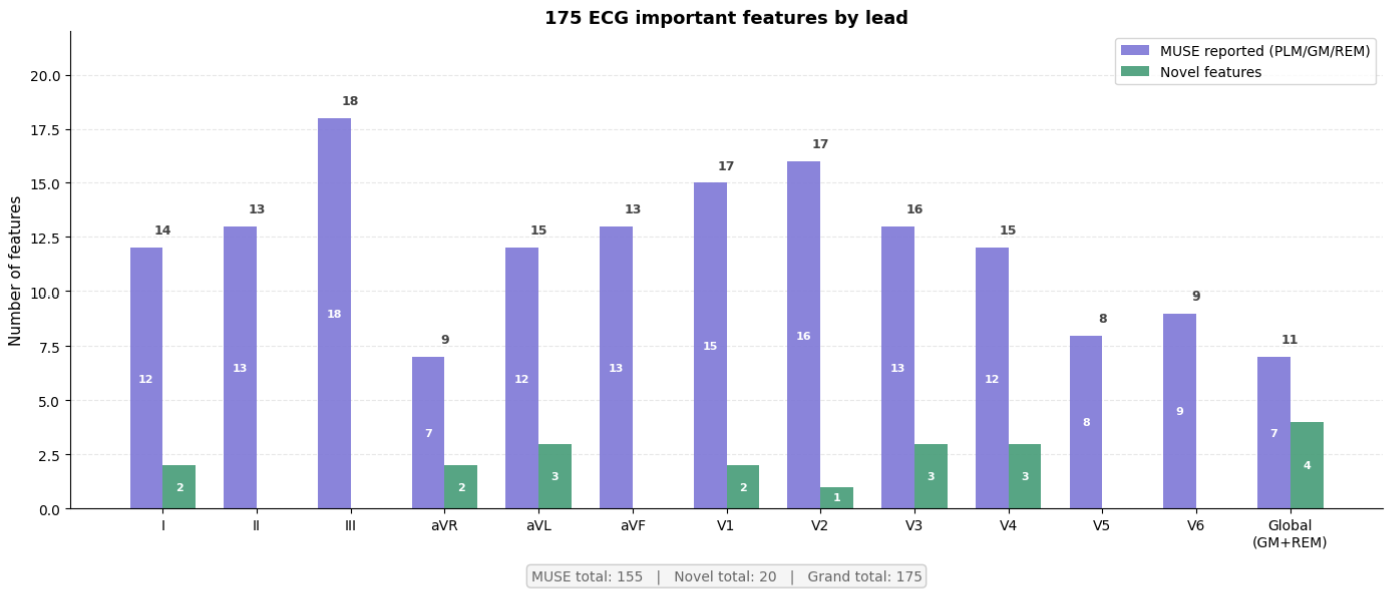
\includegraphics[width=0.98\textwidth,height=6.0cm,keepaspectratio]{leadimportance.png}
  \end{beamercolorbox}
\end{frame}


  

% ---------- Subsection Slide: Final Sequential Feature Importance ----------
\begin{frame}{Decision-Tree Modeling --- Final Feature Importance}
  \centering
  \vspace{-0.3em} % Pulls content up to utilize top margins
  {\small\Raleway\bfseries\color{aggieblue} Final Active Modeling Features}\\[0.4em]
  
  % Maximizes the bar chart to span the full width of the slide text block
  \makebox[\textwidth][c]{%
    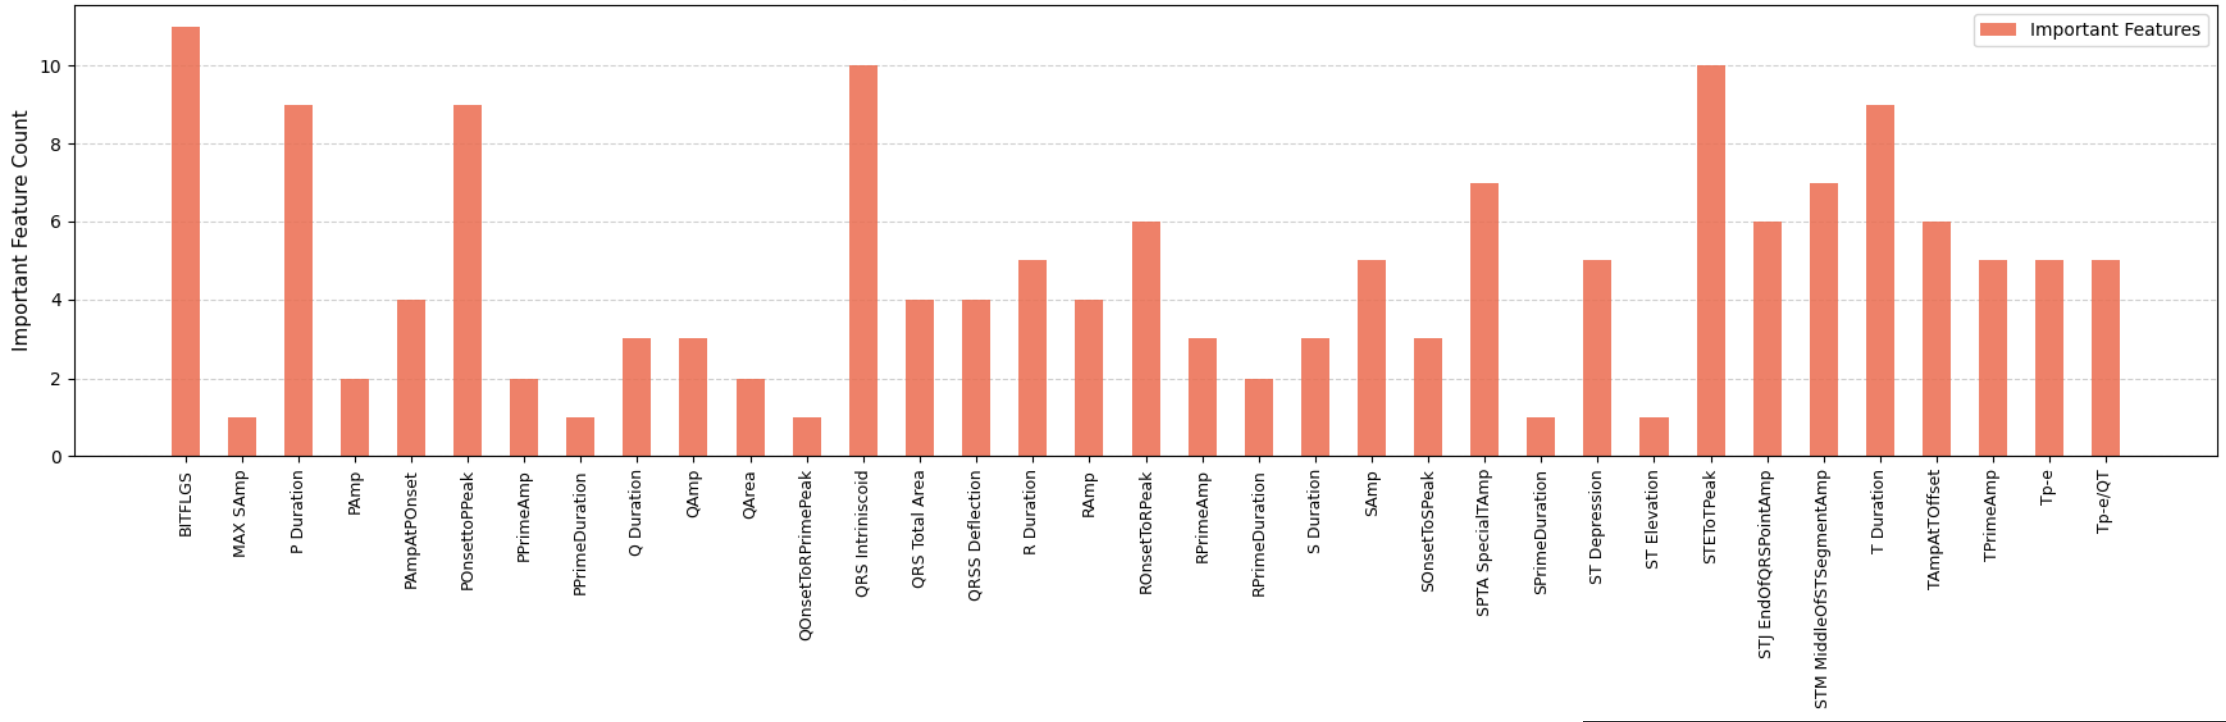
\includegraphics[width=1.03\textwidth,height=3.8cm,keepaspectratio]{finalimportance.png}
  }
  
  \vspace{0.5em} % Spacing between chart and features row
  
  % Three separate structured boxes mapping the key predictors
  \begin{columns}[T, onlytextwidth]
    
    % Box 1: Highest Seen Features
    \begin{column}{0.31\textwidth}
      \begin{beamercolorbox}[wd=\textwidth,rounded=true,shadow=false,sep=0.4em]{boxgray}
        \usebeamerfont{footline}\color{coolgray}
        \centering{\textbf{\color{aggieblue}Most Frequent}}\par
        \vspace{0.4em}
        \scriptsize
        \textbf{BITFLGS}, QRS Intrinsicoid, and STEtoTPeak
      \end{beamercolorbox}
    \end{column}
    
    \hfill
    
    % Box 2: NeuroKit Local Features
    \begin{column}{0.31\textwidth}
      \begin{beamercolorbox}[wd=\textwidth,rounded=true,shadow=false,sep=0.4em]{boxgray}
        \usebeamerfont{footline}\color{coolgray}
        \centering{\textbf{\color{aggieblue}NeuroKit -  Lead}}\par
        \vspace{0.4em}
        \scriptsize
        Tp-e, Tp-e/QT, and ST Depression
      \end{beamercolorbox}
    \end{column}
    
    \hfill
    
    % Box 3: Surviving Global Features
    \begin{column}{0.31\textwidth}
      \begin{beamercolorbox}[wd=\textwidth,rounded=true,shadow=false,sep=0.4em]{boxgray}
        \usebeamerfont{footline}\color{coolgray}
        \centering{\textbf{\color{aggieblue}NeuroKit - Global}}\par
        \vspace{0.4em}
        \scriptsize
        $P_{\max}$, $P_{\min}$, T Axis, and Frontal QRS-T Angle
      \end{beamercolorbox}
    \end{column}
    
  \end{columns}
\end{frame}

% ---------- Subsection Slide: Model Performance Comparison ----------
\begin{frame}{Decision-Tree Modeling --- Individual vs. Ensemble Performance}

  % Tighten padding to give the wide table arrays maximum clearance
  \setlength{\tabcolsep}{5pt}
  \vspace{-0.5em}

  % Top Section: Wide horizontal commentary text box
  \begin{beamercolorbox}[wd=\textwidth,rounded=true,shadow=false,sep=0.4em]{boxgray}
    \begin{itemize}
      \item \textbf{Weights:} based on AUPRC/sensitivity
      \item\textbf{RandomizedSearchCV}
    \end{itemize}
  \end{beamercolorbox}

  \vspace{0.4em}

  % Middle Section: Full-Width Standalone Base Models Table
  \centering
  {\scriptsize\Raleway\bfseries\color{aggieblue} Individual Tree-Based Classifiers}\\[0.2em]
  \begin{beamercolorbox}[wd=\textwidth,rounded=true,shadow=false,sep=0.3em]{boxgray}
    \tiny
    \resizebox{\textwidth}{!}{%
      \begin{tabular}{lcccccc}
        \textbf{Model} & \textbf{AUROC} & \textbf{AUPRC} & \textbf{Specificity} & \textbf{Sensitivity} & \textbf{Balanced Accuracy} & \textbf{F1-Score} \\
        \hline
        RandomForest & $74.49 \pm 3.77$ & $42.56 \pm 7.60$ & $74.37 \pm 3.20$ & $61.43 \pm 11.36$ & $67.90 \pm 4.30$ & $40.10 \pm 3.86$ \\
        LightGBM     & $73.25 \pm 3.47$ & $37.30 \pm 7.47$ & $72.95 \pm 4.33$ & $59.62 \pm 9.49$  & $66.28 \pm 2.62$ & $38.24 \pm 1.88$ \\
        XGBoost      & $74.84 \pm 4.50$ & $40.76 \pm 7.14$ & $74.26 \pm 3.76$ & $61.44 \pm 11.11$ & $67.85 \pm 4.28$ & $40.09 \pm 3.93$ \\
        CatBoost     & $74.55 \pm 4.94$ & $42.24 \pm 8.67$ & $75.96 \pm 4.81$ & $60.53 \pm 13.37$ & $68.24 \pm 4.56$ & $41.70 \pm 3.90$ \\
        AdaBoost     & $69.86 \pm 4.43$ & $33.91 \pm 7.71$ & $67.92 \pm 7.96$ & $59.90 \pm 13.17$ & $63.91 \pm 3.04$ & $35.14 \pm 2.44$ \\
      \end{tabular}%
    }
  \end{beamercolorbox}

  \vspace{0.4em}

  % Bottom Section: Full-Width Ensemble Architectures Table
  {\scriptsize\Raleway\bfseries\color{aggieblue} Multi-Model Ensemble}\\[0.2em]
  \begin{beamercolorbox}[wd=\textwidth,rounded=true,shadow=false,sep=0.3em]{boxgray}
    \tiny
    \resizebox{\textwidth}{!}{%
      \begin{tabular}{lcccccc}
        \textbf{Ensemble} & \textbf{AUROC} & \textbf{AUPRC} & \textbf{Specificity} & \textbf{Sensitivity} & \textbf{Balanced Accuracy} & \textbf{F1-Score} \\
        \hline
        Unweighted Voting  & $74.54 \pm 4.16$ & $41.81 \pm 7.86$ & $74.26 \pm 3.95$ & $59.32 \pm 10.70$ & $66.79 \pm 3.60$ & $38.94 \pm 2.99$ \\
        Weighted Voting    & $74.75 \pm 4.35$ & $42.26 \pm 7.92$ & $74.75 \pm 4.48$ & $60.23 \pm 10.88$ & $67.49 \pm 3.45$ & $39.80 \pm 2.76$ \\
        \textbf{Unweighted Voting+} & $\mathbf{75.72 \pm 3.94}$ & $41.58 \pm 8.03$ & $74.64 \pm 4.70$ & $\mathbf{62.35 \pm 10.93}$ & $\mathbf{68.50 \pm 3.22}$ & $40.85 \pm 2.24$ \\
        Stacking           & $74.77 \pm 4.35$ & $42.43 \pm 7.59$ & $74.37 \pm 4.18$ & $59.62 \pm 10.80$ & $67.00 \pm 3.46$ & $39.17 \pm 2.79$ \\
        Bagging CatBoost   & $74.81 \pm 4.98$ & $41.96 \pm 8.86$ & $74.70 \pm 4.68$ & $59.62 \pm 15.19$ & $67.16 \pm 5.59$ & $39.10 \pm 5.21$ \\
      \end{tabular}%
    }
  \end{beamercolorbox}

\end{frame}

% ---------- Subsection Slide: 6 Lead Progression ----------
\begin{frame}{Decision-Tree Modeling --- 6 Lead Progression}

  \begin{columns}[T, onlytextwidth]

    % Left Column: Methodology (40% width)
    \begin{column}{0.40\textwidth}
      \vspace{0.2em}
      \usebeamerfont{footline}\color{coolgray}
      \begin{itemize}
        \item StratifiedGroupKFold, $k = 10$
        \item ReliefF as a feature selector
        \item Boruta as second feature selector
        \item Feature Importance with CatBoost
        \item Based off of which lead's features came up the most, picked leads I, III, V1, V3, V5, and AVL
      \end{itemize}
    \end{column}

    % Right Column: Performance Table (57% width)
    \begin{column}{0.57\textwidth}
      \centering
      {\scriptsize\Raleway\bfseries\color{aggieblue} 6 Lead Progression Results}\\[0.3em]
      \begin{beamercolorbox}[wd=\textwidth,rounded=true,leftskip=0.2em,rightskip=0.2em,sep=0.4em]{boxgray}
        \small
        \resizebox{\textwidth}{!}{
          \begin{tabular}{lcc}
            \textbf{Metric} & \textbf{12 Leads} & \textbf{6 Leads} \\
            \hline
            Balanced Accuracy & $0.644 \pm 0.113$ & $0.63 \pm 0.077$ \\
            Precision & $0.66 \pm 0.18$ & $0.64 \pm 0.13$ \\
            Recall & $0.61 \pm 0.16$ & $0.60 \pm 0.13$ \\
            F1 Score & $0.62 \pm 0.14$ & $0.61 \pm 0.11$ \\
            ROC-AUC & $0.64 \pm 0.11$ & $0.63 \pm 0.08$ \\
          \end{tabular}
        }
      \end{beamercolorbox}
    \end{column}

  \end{columns}
\end{frame}

% ==========================================================================
% CNN / TRANSFORMER ARCHITECTURE SECTION
% ==========================================================================

% ---------- Transition Slide: Neural Network Modeling ----------
{%
  \setbeamertemplate{footline}{}%
  \begin{frame}[plain,noframenumbering]
    \begin{tikzpicture}[remember picture,overlay]
      \fill[aggieblue] (current page.south west) rectangle (current page.north east);
    \end{tikzpicture}
    \vfill
    \centering
    {\Raleway\bfseries\Huge\color{white} Neural Network Modeling}\\[0.6em]
    {\color{aggiegold}\rule{6cm}{0.06cm}}
    \vfill
  \end{frame}
}

% ---------- Subsection Slide: Preprocessing & Training ----------
\begin{frame}{Neural Network Modeling --- Preprocessing \& Training}
  \begin{columns}[T]

    \begin{column}{0.48\textwidth}
      \centering
      {\small\Raleway\bfseries\color{aggieblue} Signal Preprocessing}\\[0.4em]
      \usebeamerfont{footline}\color{coolgray}
      Three steps applied per-lead in order:
      \begin{enumerate}
        \item \textbf{Baseline Wander Removal:} 4th-order Butterworth high-pass at 0.5~Hz, zero-phase SOS form
        \item \textbf{Powerline Interference:} 60~Hz IIR notch filter ($Q=30$); notch width $\sim$2~Hz
        \item \textbf{Z-Score Normalization:} Per-lead $\frac{x - \mu_\ell}{\sigma_\ell + \epsilon}$
      \end{enumerate}
    \end{column}

    \begin{column}{0.48\textwidth}
      {\small\Raleway\bfseries\color{aggieblue} Training Configuration}\\[0.4em]
      \usebeamerfont{footline}\color{coolgray}
      \begin{itemize}
        \item \textbf{AdamW} optimizer + cosine annealing (lr $= 2\!\times\!10^{-3}$)
        \item Dropout 0.15, weight decay $5\!\times\!10^{-3}$
        \item Label smoothing 0.05 + mixup ($\alpha = 0.2$)
        \item Early stop on val AUROC, patience 20, up to 80 epochs
        \item StratifiedGroupKFold ($k = 5$), 20 seeds, 5-bag ensemble
      \end{itemize}
    \end{column}

  \end{columns}

  \vspace{0.5em}
  {\small\Raleway\bfseries\color{aggieblue}\centering 7-Transform On-the-Fly Augmentation\par}\vspace{0.3em}
  \resizebox{\textwidth}{!}{%
    \begin{tabular}{llll}
      \toprule
      \textbf{Transform} & \textbf{Prob.} & \textbf{Range} & \textbf{Description} \\
      \midrule
      Gaussian Noise & 50\% & $\sigma \in [0.01, 0.05]$ & Adds random noise to all leads; simulates sensor/environmental noise \\
      Amplitude Scale & 50\% & $\pm 15\%$ & Randomly scales signal amplitude; models gain variation across devices \\
      Time Shift & 30\% & $\pm 150$ samples & Circularly shifts the waveform in time ($\pm$0.6\,s at 250\,Hz) \\
      Lead Dropout & 10\% & 12\% per lead & When triggered, each lead is independently zeroed; forces cross-lead redundancy \\
      Cutout & 25\% & 50--200 samples & Zeros a contiguous random segment across all leads; prevents reliance on any single region \\
      Baseline Wander & 20\% & 0.05--0.5~Hz & Injects a low-frequency sinusoid; simulates electrode drift or patient motion \\
      Speed Perturb & 10\% & $\pm 5\%$ & Resamples to stretch/compress the signal; models heart-rate variability \\
      \bottomrule
    \end{tabular}
  }%
  \vspace{0.2em}
  {\scriptsize\Lato\color{coolgray}\centering Applied stochastically per sample during training. Class balance via \textbf{WeightedRandomSampler}.\par}
\end{frame}

% ---------- Subsection Slide: Depthwise Separable Convolution ----------
\begin{frame}{Neural Network Modeling --- Multi-Scale Depthwise Separable Conv (Stage 1)}
  \centering
  \vspace{-0.3em}
  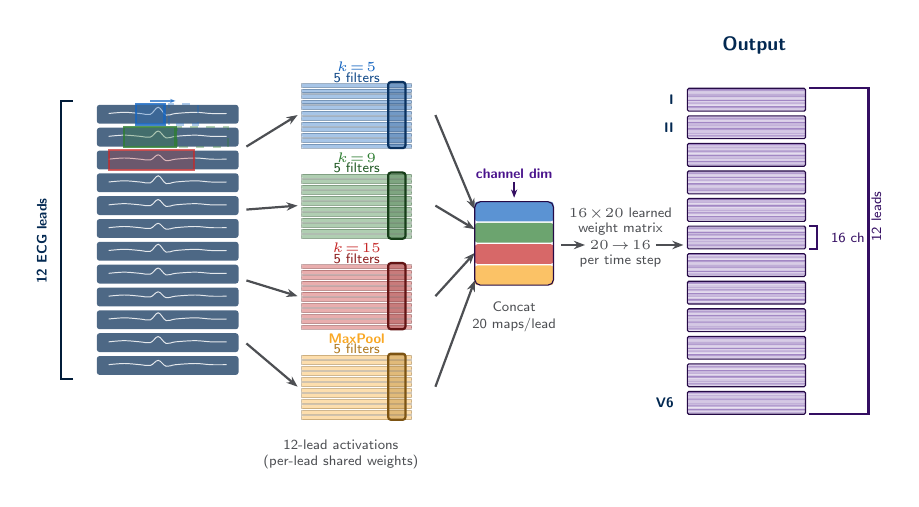
\begin{tikzpicture}[
    x=1cm, y=1cm,
    arr/.style={-{Stealth[length=4pt]}, thick, coolgray},
    lbl/.style={font=\scriptsize\bfseries, text=aggieblue, align=center},
    sublbl/.style={font=\tiny, text=coolgray, align=center},
  ]
    \definecolor{br1}{HTML}{1565C0}
    \definecolor{br2}{HTML}{2E7D32}
    \definecolor{br3}{HTML}{C62828}
    \definecolor{br4}{HTML}{F9A825}
    \definecolor{outc}{HTML}{4A148C}

    % ===== INPUT: 12 ECG lead bars with waveforms =====
    \foreach \i in {0,...,11}{
      \pgfmathsetmacro{\ypos}{\i * 0.29}
      \pgfmathsetmacro{\ymid}{\ypos + 0.13}
      \pgfmathsetmacro{\amp}{0.055 + mod(\i, 3) * 0.012}
      \fill[aggieblue, opacity=0.7, rounded corners=1pt] (0, \ypos) rectangle ++(1.8, 0.24);
      \draw[white, opacity=0.85, line width=0.35pt]
        plot[smooth, tension=0.6] coordinates {
          (0.15, \ymid)
          (0.35, {\ymid+0.015})
          (0.55, \ymid)
          (0.68, {\ymid-0.01})
          (0.78, {\ymid+\amp})
          (0.88, {\ymid-0.02})
          (1.0,  \ymid)
          (1.25, {\ymid+0.015})
          (1.45, \ymid)
          (1.65, \ymid)
        };
    }

    % --- Kernel windows superimposed on leads ---
    % k=5 on Lead I (index 11): narrow blue window + ghost showing slide
    \fill[br1, opacity=0.3] (0.5, {11*0.29-0.01}) rectangle ++(0.36, 0.26);
    \draw[br1, thick, opacity=0.8] (0.5, {11*0.29-0.01}) rectangle ++(0.36, 0.26);
    \draw[br1, dashed, thick, opacity=0.35] (0.92, {11*0.29-0.01}) rectangle ++(0.36, 0.26);
    \draw[-{Stealth[length=2pt]}, br1, thick, opacity=0.7]
      (0.68, {11*0.29+0.29}) -- ++(0.32, 0);

    % k=9 on Lead II (index 10): medium green window
    \fill[br2, opacity=0.3] (0.35, {10*0.29-0.01}) rectangle ++(0.65, 0.26);
    \draw[br2, thick, opacity=0.8] (0.35, {10*0.29-0.01}) rectangle ++(0.65, 0.26);
    \draw[br2, dashed, thick, opacity=0.35] (1.02, {10*0.29-0.01}) rectangle ++(0.65, 0.26);

    % k=15 on Lead III (index 9): wide red window
    \fill[br3, opacity=0.25] (0.15, {9*0.29-0.01}) rectangle ++(1.08, 0.26);
    \draw[br3, thick, opacity=0.7] (0.15, {9*0.29-0.01}) rectangle ++(1.08, 0.26);

    % Lead labels
    \node[font=\fontsize{3.5}{4}\selectfont\bfseries, text=white, anchor=east]
      at (-0.08, {11*0.29+0.13}) {I};
    \node[font=\fontsize{3.5}{4}\selectfont\bfseries, text=white, anchor=east]
      at (-0.08, {10*0.29+0.13}) {II};
    \node[font=\fontsize{3.5}{4}\selectfont\bfseries, text=white, anchor=east]
      at (-0.08, {9*0.29+0.13}) {III};
    \node[font=\fontsize{3.5}{4}\selectfont\bfseries, text=white, anchor=east]
      at (-0.08, {5*0.29+0.13}) {V1};
    \node[font=\fontsize{3.5}{4}\selectfont\bfseries, text=white, anchor=east]
      at (-0.08, {0*0.29+0.13}) {V6};
    % Bracket
    \draw[aggieblue!70!black, thick] (-0.3, -0.05) -- (-0.45, -0.05)
      -- (-0.45, {11*0.29+0.24+0.05}) -- (-0.3, {11*0.29+0.24+0.05});
    \node[font=\fontsize{4}{5}\selectfont\bfseries, text=aggieblue, rotate=90]
      at (-0.7, 1.7) {12 ECG leads};

    % ===== FOUR BRANCHES — 12-lead activations + PW overlay → output =====
    % Branch y-centers: 3.3, 2.15, 1.0, -0.15
    % 12 bars per branch: 0.07 spacing x 12 = 0.84 height

    % Arrows from input to branches
    \draw[arr] (1.9, 2.9) -- (2.55, 3.3);
    \draw[arr] (1.9, 2.1) -- (2.55, 2.15);
    \draw[arr] (1.9, 1.2) -- (2.55, 1.0);
    \draw[arr] (1.9, 0.4) -- (2.55, -0.15);

    % --- Branch 1: k=5 (center y=3.3, bars y=2.88..3.72) ---
    \node[font=\fontsize{5}{6}\selectfont\bfseries, text=br1]
      at (3.3, 3.91) {$k\!=\!5$};
    \node[font=\fontsize{3.5}{4}\selectfont, text=br1!70!black]
      at (3.3, 3.78) {5 filters};
    \foreach \j in {0,...,11}{
      \pgfmathsetmacro{\by}{2.88 + \j * 0.07}
      \fill[br1!50!white, opacity=0.75, rounded corners=0.5pt] (2.6, \by) rectangle ++(1.4, 0.05);
      \draw[br1!40!black, opacity=0.3] (2.6, \by) rectangle ++(1.4, 0.05);
    }
    \fill[br1!70!black, opacity=0.35] (3.7, 2.88) rectangle ++(0.22, 0.84);
    \draw[br1!50!black, thick, rounded corners=1pt] (3.7, 2.88) rectangle ++(0.22, 0.84);

    % --- Branch 2: k=9 (center y=2.15, bars y=1.73..2.57) ---
    \node[font=\fontsize{5}{6}\selectfont\bfseries, text=br2]
      at (3.3, 2.76) {$k\!=\!9$};
    \node[font=\fontsize{3.5}{4}\selectfont, text=br2!70!black]
      at (3.3, 2.63) {5 filters};
    \foreach \j in {0,...,11}{
      \pgfmathsetmacro{\by}{1.73 + \j * 0.07}
      \fill[br2!50!white, opacity=0.75, rounded corners=0.5pt] (2.6, \by) rectangle ++(1.4, 0.05);
      \draw[br2!40!black, opacity=0.3] (2.6, \by) rectangle ++(1.4, 0.05);
    }
    \fill[br2!70!black, opacity=0.35] (3.7, 1.73) rectangle ++(0.22, 0.84);
    \draw[br2!50!black, thick, rounded corners=1pt] (3.7, 1.73) rectangle ++(0.22, 0.84);

    % --- Branch 3: k=15 (center y=1.0, bars y=0.58..1.42) ---
    \node[font=\fontsize{5}{6}\selectfont\bfseries, text=br3]
      at (3.3, 1.61) {$k\!=\!15$};
    \node[font=\fontsize{3.5}{4}\selectfont, text=br3!70!black]
      at (3.3, 1.48) {5 filters};
    \foreach \j in {0,...,11}{
      \pgfmathsetmacro{\by}{0.58 + \j * 0.07}
      \fill[br3!50!white, opacity=0.75, rounded corners=0.5pt] (2.6, \by) rectangle ++(1.4, 0.05);
      \draw[br3!40!black, opacity=0.3] (2.6, \by) rectangle ++(1.4, 0.05);
    }
    \fill[br3!70!black, opacity=0.35] (3.7, 0.58) rectangle ++(0.22, 0.84);
    \draw[br3!50!black, thick, rounded corners=1pt] (3.7, 0.58) rectangle ++(0.22, 0.84);

    % --- Branch 4: MaxPool (center y=-0.15, bars y=-0.57..0.27) ---
    \node[font=\fontsize{4.5}{5.5}\selectfont\bfseries, text=br4]
      at (3.3, 0.46) {MaxPool};
    \node[font=\fontsize{3.5}{4}\selectfont, text=br4!70!black]
      at (3.3, 0.33) {5 filters};
    \foreach \j in {0,...,11}{
      \pgfmathsetmacro{\by}{-0.57 + \j * 0.07}
      \fill[br4!50!white, opacity=0.75, rounded corners=0.5pt] (2.6, \by) rectangle ++(1.4, 0.05);
      \draw[br4!40!black, opacity=0.3] (2.6, \by) rectangle ++(1.4, 0.05);
    }
    \fill[br4!70!black, opacity=0.35] (3.7, -0.57) rectangle ++(0.22, 0.84);
    \draw[br4!50!black, thick, rounded corners=1pt] (3.7, -0.57) rectangle ++(0.22, 0.84);

    % Inline labels below bottom branch
    \node[sublbl, below] at (3.1, -0.7) {12-lead activations};
    \node[sublbl, below] at (3.1, -0.9) {(per-lead shared weights)};

    % ===== CONCAT =====
    \draw[arr] (4.3, 3.3) -- (4.8, 2.1);
    \draw[arr] (4.3, 2.15) -- (4.8, 1.85);
    \draw[arr] (4.3, 1.0) -- (4.8, 1.55);
    \draw[arr] (4.3, -0.15) -- (4.8, 1.2);

    \fill[br1, opacity=0.7, rounded corners=1pt] (4.8, 1.95) rectangle ++(1.0, 0.25);
    \fill[br2, opacity=0.7, rounded corners=1pt] (4.8, 1.68) rectangle ++(1.0, 0.25);
    \fill[br3, opacity=0.7, rounded corners=1pt] (4.8, 1.41) rectangle ++(1.0, 0.25);
    \fill[br4, opacity=0.7, rounded corners=1pt] (4.8, 1.14) rectangle ++(1.0, 0.25);
    \draw[outc!50!black, rounded corners=2pt] (4.8, 1.14) rectangle ++(1.0, 1.06);
    \draw[-{Stealth[length=3pt]}, outc!70!black, thick]
      (5.3, 2.45) -- (5.3, 2.25);
    \node[font=\fontsize{4}{5}\selectfont\bfseries, text=outc]
      at (5.3, 2.55) {channel dim};
    \node[sublbl, below] at (5.3, 1.05) {Concat};
    \node[sublbl, below] at (5.3, 0.85) {20 maps/lead};

    % ===== 1x1 projection =====
    \draw[arr] (5.9, 1.65) -- (6.2, 1.65);
    \node[sublbl] at (6.65, 2.05) {$16\!\times\!20$ learned};
    \node[sublbl] at (6.65, 1.85) {weight matrix};
    \node[sublbl] at (6.65, 1.65) {$20\!\to\!16$};
    \node[sublbl] at (6.65, 1.45) {per time step};

    % ===== Arrow from 1x1 to output =====
    \draw[arr] (7.1, 1.65) -- (7.45, 1.65);

    % ===== OUTPUT: 12 leads stacked vertically, each a block of 16 channel bars =====
    \node[lbl, above] at (8.35, 3.95) {Output};

    \foreach \lead in {0,...,11}{
      \pgfmathsetmacro{\leadbase}{-0.5 + \lead * 0.35}
      \foreach \c in {0,...,15}{
        \pgfmathsetmacro{\cy}{\leadbase + \c * 0.018}
        \pgfmathsetmacro{\opacity}{0.4 + mod(\c, 4) * 0.15}
        \fill[outc!60!white, opacity=\opacity, rounded corners=0.3pt] (7.5, \cy) rectangle ++(1.5, 0.014);
      }
      \draw[outc!50!black, rounded corners=0.5pt] (7.5, \leadbase) rectangle ++(1.5, 0.29);
    }

    % Lead labels on a few
    \node[font=\fontsize{3.5}{4}\selectfont\bfseries, text=aggieblue, anchor=east]
      at (7.45, {-0.5 + 11*0.35 + 0.145}) {I};
    \node[font=\fontsize{3.5}{4}\selectfont\bfseries, text=aggieblue, anchor=east]
      at (7.45, {-0.5 + 10*0.35 + 0.145}) {II};
    \node[font=\fontsize{3.5}{4}\selectfont\bfseries, text=aggieblue, anchor=east]
      at (7.45, {-0.5 + 0*0.35 + 0.145}) {V6};

    % Bracket showing 16 ch on a middle lead (lead index 6)
    \draw[outc!70!black, thick] (9.05, {-0.5 + 6*0.35}) -- (9.15, {-0.5 + 6*0.35})
      -- (9.15, {-0.5 + 6*0.35 + 0.29}) -- (9.05, {-0.5 + 6*0.35 + 0.29});
    \node[font=\fontsize{3.5}{4}\selectfont, text=outc!70!black, anchor=west]
      at (9.2, {-0.5 + 6*0.35 + 0.145}) {16 ch};

    % Bracket showing 12 leads on right (outer bracket)
    \draw[outc!70!black, thick] (9.05, {-0.5}) -- (9.8, {-0.5})
      -- (9.8, {-0.5 + 11*0.35 + 0.29}) -- (9.05, {-0.5 + 11*0.35 + 0.29});
    \node[font=\fontsize{3.5}{4}\selectfont, text=outc!70!black, anchor=west, rotate=90]
      at (9.9, {-0.5 + 5.5*0.35 + 0.145}) {12 leads};

  \end{tikzpicture}

  \vspace{0.3em}
  {\usebeamerfont{footline}\color{coolgray}
  Each branch runs 5 learned filters per lead (shared weights across all 12 leads) \textbullet{}
  Outputs stacked into 20 maps per lead \textbullet{}
  $1\!\times\!1$ conv learns a linear blend of all scales $\to$ 16 features per lead}
\end{frame}

% ---------- Subsection Slide: Squeeze-Excitation ----------
\begin{frame}{Neural Network Modeling --- Squeeze-Excitation (SE) Block}
  \centering
  \vspace{-0.3em}
  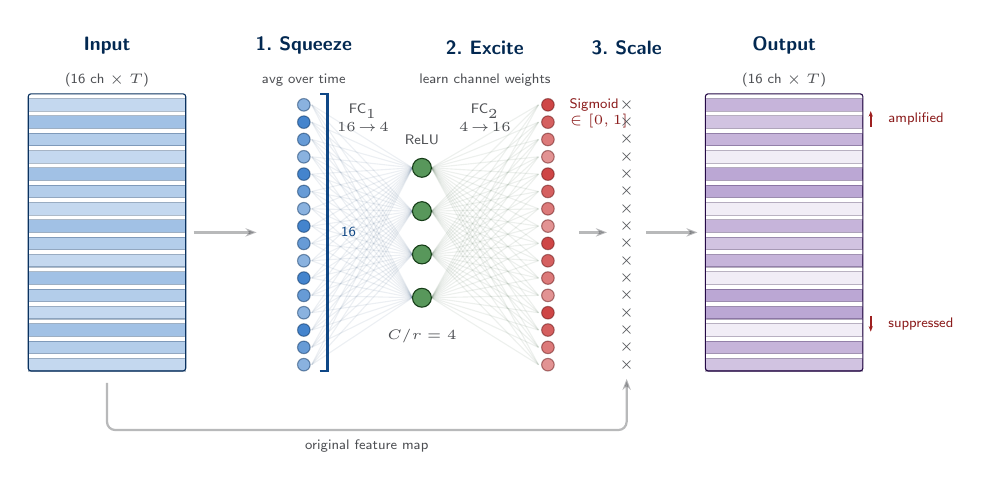
\begin{tikzpicture}[
    x=1cm, y=1cm,
    arr/.style={-{Stealth[length=4pt]}, thick, coolgray},
    lbl/.style={font=\scriptsize\bfseries, text=aggieblue, align=center},
    sublbl/.style={font=\tiny, text=coolgray, align=center},
  ]
    \definecolor{sec}{HTML}{1565C0}
    \definecolor{bot}{HTML}{2E7D32}
    \definecolor{wt}{HTML}{C62828}
    \definecolor{outc}{HTML}{4A148C}

    % ===== INPUT: 16 channel bars (one lead's feature map) =====
    \node[lbl, above] at (1.0, 4.1) {Input};
    \node[sublbl] at (1.0, 3.9) {(16 ch $\times$ $T$)};

    \foreach \c in {0,...,15}{
      \pgfmathsetmacro{\cy}{0.2 + \c * 0.22}
      \pgfmathsetmacro{\opacity}{0.5 + mod(\c, 3) * 0.15}
      \fill[sec!50!white, opacity=\opacity, rounded corners=0.5pt] (0, \cy) rectangle ++(2.0, 0.16);
      \draw[sec!40!black, opacity=0.3] (0, \cy) rectangle ++(2.0, 0.16);
    }
    \draw[sec!50!black, rounded corners=1pt] (0, 0.2) rectangle ++(2.0, 3.52);

    % ===== STEP 1: SQUEEZE — Global Average Pool =====
    \node[lbl, above] at (3.5, 4.1) {1.\ Squeeze};
    \node[sublbl] at (3.5, 3.9) {avg over time};

    % Arrows from input bars to scalar dots
    \draw[arr, opacity=0.4] (2.1, 1.96) -- (2.9, 1.96);

    % 16 scalar circles (compressed channel values)
    \foreach \c in {0,...,15}{
      \pgfmathsetmacro{\cy}{0.2 + \c * 0.22 + 0.08}
      \pgfmathsetmacro{\opacity}{0.5 + mod(\c, 3) * 0.15}
      \fill[sec, opacity=\opacity] (3.5, \cy) circle (0.08);
      \draw[sec!50!black, opacity=0.5] (3.5, \cy) circle (0.08);
    }

    % Bracket: 16 scalars
    \draw[sec!70!black, thick] (3.7, 0.2) -- (3.8, 0.2)
      -- (3.8, 3.72) -- (3.7, 3.72);
    \node[font=\fontsize{3.5}{4}\selectfont, text=sec!70!black, anchor=west]
      at (3.85, 1.96) {16};

    % ===== STEP 2: EXCITE — FC bottleneck =====
    \node[lbl, above] at (5.8, 4.1) {2.\ Excite};
    \node[sublbl] at (5.8, 3.9) {learn channel weights};

    % FC1 label
    \node[sublbl] at (4.25, 3.5) {FC$_1$};
    \node[font=\fontsize{3}{3.5}\selectfont, text=coolgray] at (4.25, 3.3) {$16\!\to\!4$};

    % Lines from ALL 16 scalars to ALL 4 bottleneck neurons (FC1)
    \foreach \c in {0,...,15}{
      \pgfmathsetmacro{\cy}{0.2 + \c * 0.22 + 0.08}
      \foreach \b in {0,...,3}{
        \pgfmathsetmacro{\by}{1.13 + \b * 0.55}
        \draw[sec!50!black, opacity=0.08] (3.6, \cy) -- (4.88, \by);
      }
    }

    % 4 bottleneck neurons
    \foreach \b in {0,...,3}{
      \pgfmathsetmacro{\by}{1.13 + \b * 0.55}
      \fill[bot, opacity=0.8] (5.0, \by) circle (0.12);
      \draw[bot!50!black] (5.0, \by) circle (0.12);
    }
    \node[sublbl, below] at (5.0, 0.85) {$C/r = 4$};
    \node[sublbl, above] at (5.0, 2.95) {ReLU};

    % FC2 label
    \node[sublbl] at (5.8, 3.5) {FC$_2$};
    \node[font=\fontsize{3}{3.5}\selectfont, text=coolgray] at (5.8, 3.3) {$4\!\to\!16$};

    % Lines from ALL 4 bottleneck to ALL 16 weights (FC2)
    \foreach \b in {0,...,3}{
      \pgfmathsetmacro{\by}{1.13 + \b * 0.55}
      \foreach \c in {0,...,15}{
        \pgfmathsetmacro{\cy}{0.2 + \c * 0.22 + 0.08}
        \draw[bot!50!black, opacity=0.08] (5.12, \by) -- (6.48, \cy);
      }
    }

    % 16 weight circles (output of FC2 + sigmoid)
    \foreach \c in {0,...,15}{
      \pgfmathsetmacro{\cy}{0.2 + \c * 0.22 + 0.08}
      \pgfmathsetmacro{\opacity}{0.5 + mod(\c, 4) * 0.12}
      \fill[wt, opacity=\opacity] (6.6, \cy) circle (0.08);
      \draw[wt!50!black, opacity=0.5] (6.6, \cy) circle (0.08);
    }

    % Sigmoid label (to the right of weight dots, not on top)
    \node[font=\fontsize{3.5}{4}\selectfont, text=wt!70!black, anchor=west]
      at (6.75, 3.58) {Sigmoid};
    \node[font=\fontsize{3}{3.5}\selectfont, text=wt!70!black, anchor=west]
      at (6.75, 3.38) {$\in [0,1]$};

    % ===== STEP 3: SCALE — channel-wise multiply =====
    \node[lbl, above] at (7.6, 4.1) {3.\ Scale};

    % Multiply symbols
    \foreach \c in {0,...,15}{
      \pgfmathsetmacro{\cy}{0.2 + \c * 0.22 + 0.08}
      \node[font=\fontsize{4}{5}\selectfont, text=coolgray] at (7.6, \cy) {$\times$};
    }

    % Arrows from weights to multiply
    \draw[arr, opacity=0.4] (7.0, 1.96) -- (7.35, 1.96);

    % Curved arrows from input to multiply (skip connection)
    \draw[arr, opacity=0.4, rounded corners=3pt]
      (1.0, 0.05) -- (1.0, -0.55) -- (7.6, -0.55) -- (7.6, 0.1);
    \node[sublbl] at (4.3, -0.75) {original feature map};

    % ===== OUTPUT: re-weighted 16 channel bars =====
    \node[lbl, above] at (9.6, 4.1) {Output};
    \node[sublbl] at (9.6, 3.9) {(16 ch $\times$ $T$)};

    % Arrow from multiply to output
    \draw[arr, opacity=0.4] (7.85, 1.96) -- (8.5, 1.96);

    \foreach \c in {0,...,15}{
      \pgfmathsetmacro{\cy}{0.2 + \c * 0.22}
      % Vary opacity to show some channels amplified, others suppressed
      \pgfmathsetmacro{\opacity}{0.15 + mod(\c*\c + 3, 7) * 0.12}
      \fill[outc!50!white, opacity=\opacity, rounded corners=0.5pt] (8.6, \cy) rectangle ++(2.0, 0.16);
      \draw[outc!40!black, opacity=0.3] (8.6, \cy) rectangle ++(2.0, 0.16);
    }
    \draw[outc!50!black, rounded corners=1pt] (8.6, 0.2) rectangle ++(2.0, 3.52);

    % Annotation: amplified vs suppressed
    \draw[-{Stealth[length=2pt]}, wt!80!black, thick] (10.7, 3.3) -- (10.7, 3.5);
    \node[font=\fontsize{3}{3.5}\selectfont, text=wt!70!black, anchor=west] at (10.8, 3.4) {amplified};
    \draw[-{Stealth[length=2pt]}, wt!80!black, thick] (10.7, 0.9) -- (10.7, 0.7);
    \node[font=\fontsize{3}{3.5}\selectfont, text=wt!70!black, anchor=west] at (10.8, 0.8) {suppressed};

  \end{tikzpicture}

  \vspace{0.3em}
  {\usebeamerfont{footline}\color{coolgray}
  Applied after every conv block (Stage~1: SE(16), Stage~2: SE(32), Stage~3: SE(64)) \textbullet{}
  Learns which feature channels matter for each sample \textbullet{}
  Suppresses noise, amplifies discriminative morphology (P-wave, ST segment, QRS)}
\end{frame}

% ---------- Subsection Slide: Multi-Head Cross-Lead Attention ----------
\begin{frame}{Neural Network Modeling --- Multi-Head Cross-Lead Attention}
  \begin{columns}[T]

    \begin{column}{0.30\textwidth}
      \centering
      {\small\Raleway\bfseries\color{aggieblue} RepNet-SE Architecture}\\[0.2em]
      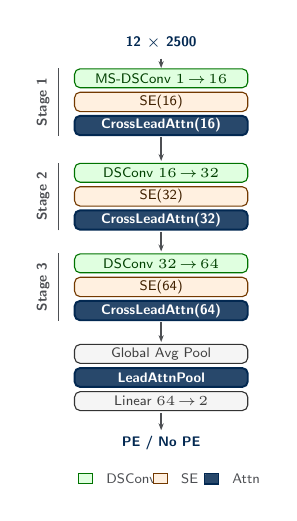
\begin{tikzpicture}[
        x=1cm, y=1cm,
        block/.style={rounded corners=2pt, minimum width=2.2cm, minimum height=0.24cm,
          font=\fontsize{4}{5}\selectfont, inner sep=1pt, align=center},
        dsblock/.style={block, fill=green!12!white, draw=green!45!black, text=green!25!black},
        seblock/.style={block, fill=orange!12!white, draw=orange!45!black, text=orange!25!black},
        attnblock/.style={block, fill=aggieblue!85!white, draw=aggieblue, line width=0.7pt,
          text=white},
        otherblock/.style={block, fill=gray!8!white, draw=gray!40!black, text=gray!50!black},
        arr/.style={-{Stealth[length=2.5pt]}, coolgray, thick},
        stglbl/.style={font=\fontsize{3.5}{4}\selectfont\bfseries, text=coolgray},
      ]
        % Input
        \node[font=\fontsize{5}{6}\selectfont\bfseries, text=aggieblue] at (0, 6.5) {12 $\times$ 2500};
        \draw[arr] (0, 6.3) -- (0, 6.18);

        % Stage 1
        \node[dsblock] (s1d) at (0, 6.05) {MS-DSConv $1\!\to\!16$};
        \node[seblock] (s1s) at (0, 5.75) {SE(16)};
        \node[attnblock] (s1a) at (0, 5.45) {\textbf{CrossLeadAttn(16)}};
        \draw[arr] (0, 5.30) -- (0, 5.0);

        % Stage 2
        \node[dsblock] (s2d) at (0, 4.85) {DSConv $16\!\to\!32$};
        \node[seblock] (s2s) at (0, 4.55) {SE(32)};
        \node[attnblock] (s2a) at (0, 4.25) {\textbf{CrossLeadAttn(32)}};
        \draw[arr] (0, 4.10) -- (0, 3.85);

        % Stage 3
        \node[dsblock] (s3d) at (0, 3.70) {DSConv $32\!\to\!64$};
        \node[seblock] (s3s) at (0, 3.40) {SE(64)};
        \node[attnblock] (s3a) at (0, 3.10) {\textbf{CrossLeadAttn(64)}};
        \draw[arr] (0, 2.95) -- (0, 2.70);

        % Fusion
        \node[otherblock] (gap) at (0, 2.55) {Global Avg Pool};
        \node[attnblock] (lap) at (0, 2.25) {\textbf{LeadAttnPool}};
        \node[otherblock] (fc)  at (0, 1.95) {Linear $64\!\to\!2$};
        \draw[arr] (0, 1.80) -- (0, 1.58);

        % Output
        \node[font=\fontsize{5}{6}\selectfont\bfseries, text=aggieblue] at (0, 1.42) {PE / No PE};

        % Stage brackets
        \draw[coolgray] (-1.30, 5.32) -- (-1.30, 6.18);
        \node[stglbl, rotate=90] at (-1.50, 5.75) {Stage 1};
        \draw[coolgray] (-1.30, 4.12) -- (-1.30, 4.98);
        \node[stglbl, rotate=90] at (-1.50, 4.55) {Stage 2};
        \draw[coolgray] (-1.30, 2.97) -- (-1.30, 3.83);
        \node[stglbl, rotate=90] at (-1.50, 3.40) {Stage 3};

        % Legend
        \fill[green!12!white, rounded corners=1pt] (-1.05, 0.90) rectangle ++(0.18, 0.13);
        \draw[green!45!black] (-1.05, 0.90) rectangle ++(0.18, 0.13);
        \node[font=\fontsize{3}{3.5}\selectfont, text=coolgray, anchor=west] at (-0.82, 0.965) {DSConv};

        \fill[orange!12!white, rounded corners=1pt] (-0.1, 0.90) rectangle ++(0.18, 0.13);
        \draw[orange!45!black] (-0.1, 0.90) rectangle ++(0.18, 0.13);
        \node[font=\fontsize{3}{3.5}\selectfont, text=coolgray, anchor=west] at (0.13, 0.965) {SE};

        \fill[aggieblue!85!white, rounded corners=1pt] (0.55, 0.90) rectangle ++(0.18, 0.13);
        \draw[aggieblue, line width=0.6pt] (0.55, 0.90) rectangle ++(0.18, 0.13);
        \node[font=\fontsize{3}{3.5}\selectfont, text=coolgray, anchor=west] at (0.78, 0.965) {Attn};
      \end{tikzpicture}
    \end{column}

    \begin{column}{0.65\textwidth}
      \centering
      {\small\Raleway\bfseries\color{aggieblue} Learned Attention Weights (50-Sample Average)}\\[0.3em]
      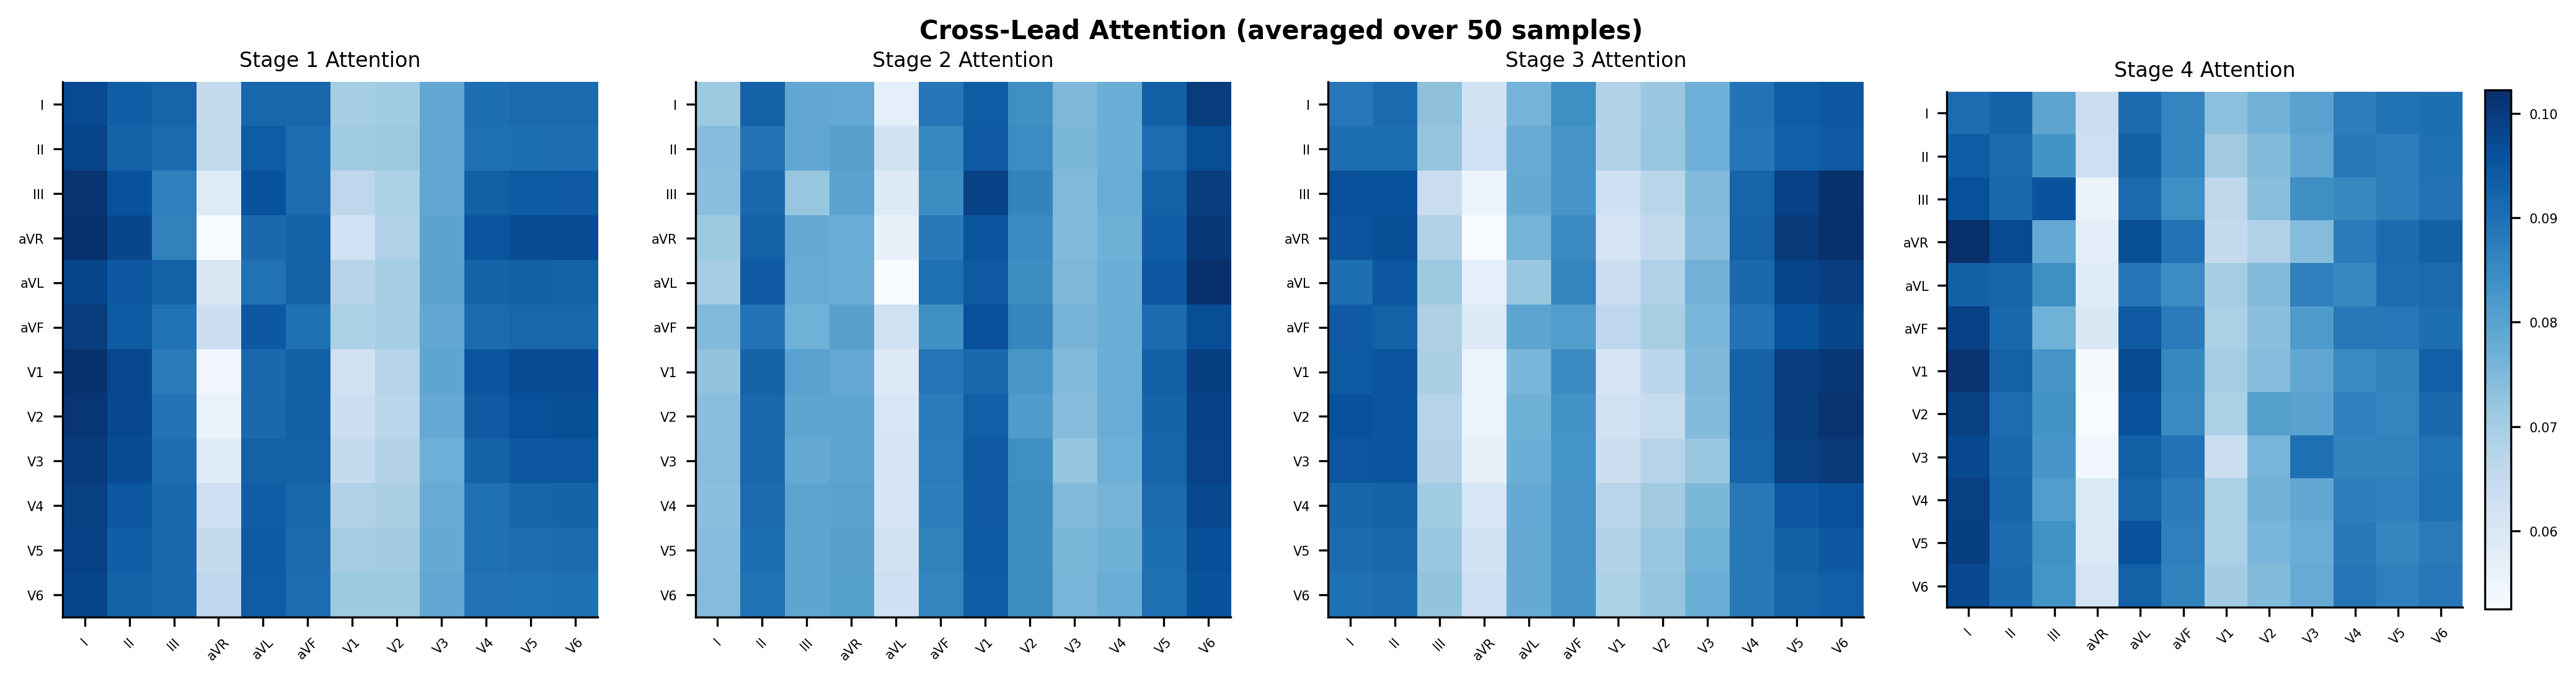
\includegraphics[width=\textwidth]{crosslead_attention_stages.png}

      \vspace{0.3em}
      \begin{itemize}\usebeamerfont{footline}\color{coolgray}
        \setlength{\itemsep}{1pt}\setlength{\parskip}{0pt}
        \item Each lead is pooled to a token; 4-head self-attention learns which leads should share information
        \item Sigmoid gating scales each lead's feature map by learned weights $\in [0,1]$ --- suppresses uninformative leads, amplifies relevant ones
        \item \textbf{Vertical stripes}: rows = query (who is looking), columns = key (who is looked at). A bright column means \textit{every} lead pulls information from that key lead --- the model treats it as a hub
        \item Weights averaged over 50 samples to reveal \textit{stable} learned patterns rather than per-sample noise
      \end{itemize}
    \end{column}

  \end{columns}
\end{frame}

% ---------- Subsection Slide: Model Performance ----------
\begin{frame}{Neural Network Modeling --- Model Performance}
  \centering
  \begin{columns}[c]
    \begin{column}{0.48\textwidth}
      \centering
      
\includegraphics[width=\textwidth]{roc_pr_curves.png}
    \end{column}
    \begin{column}{0.48\textwidth}
      \centering
      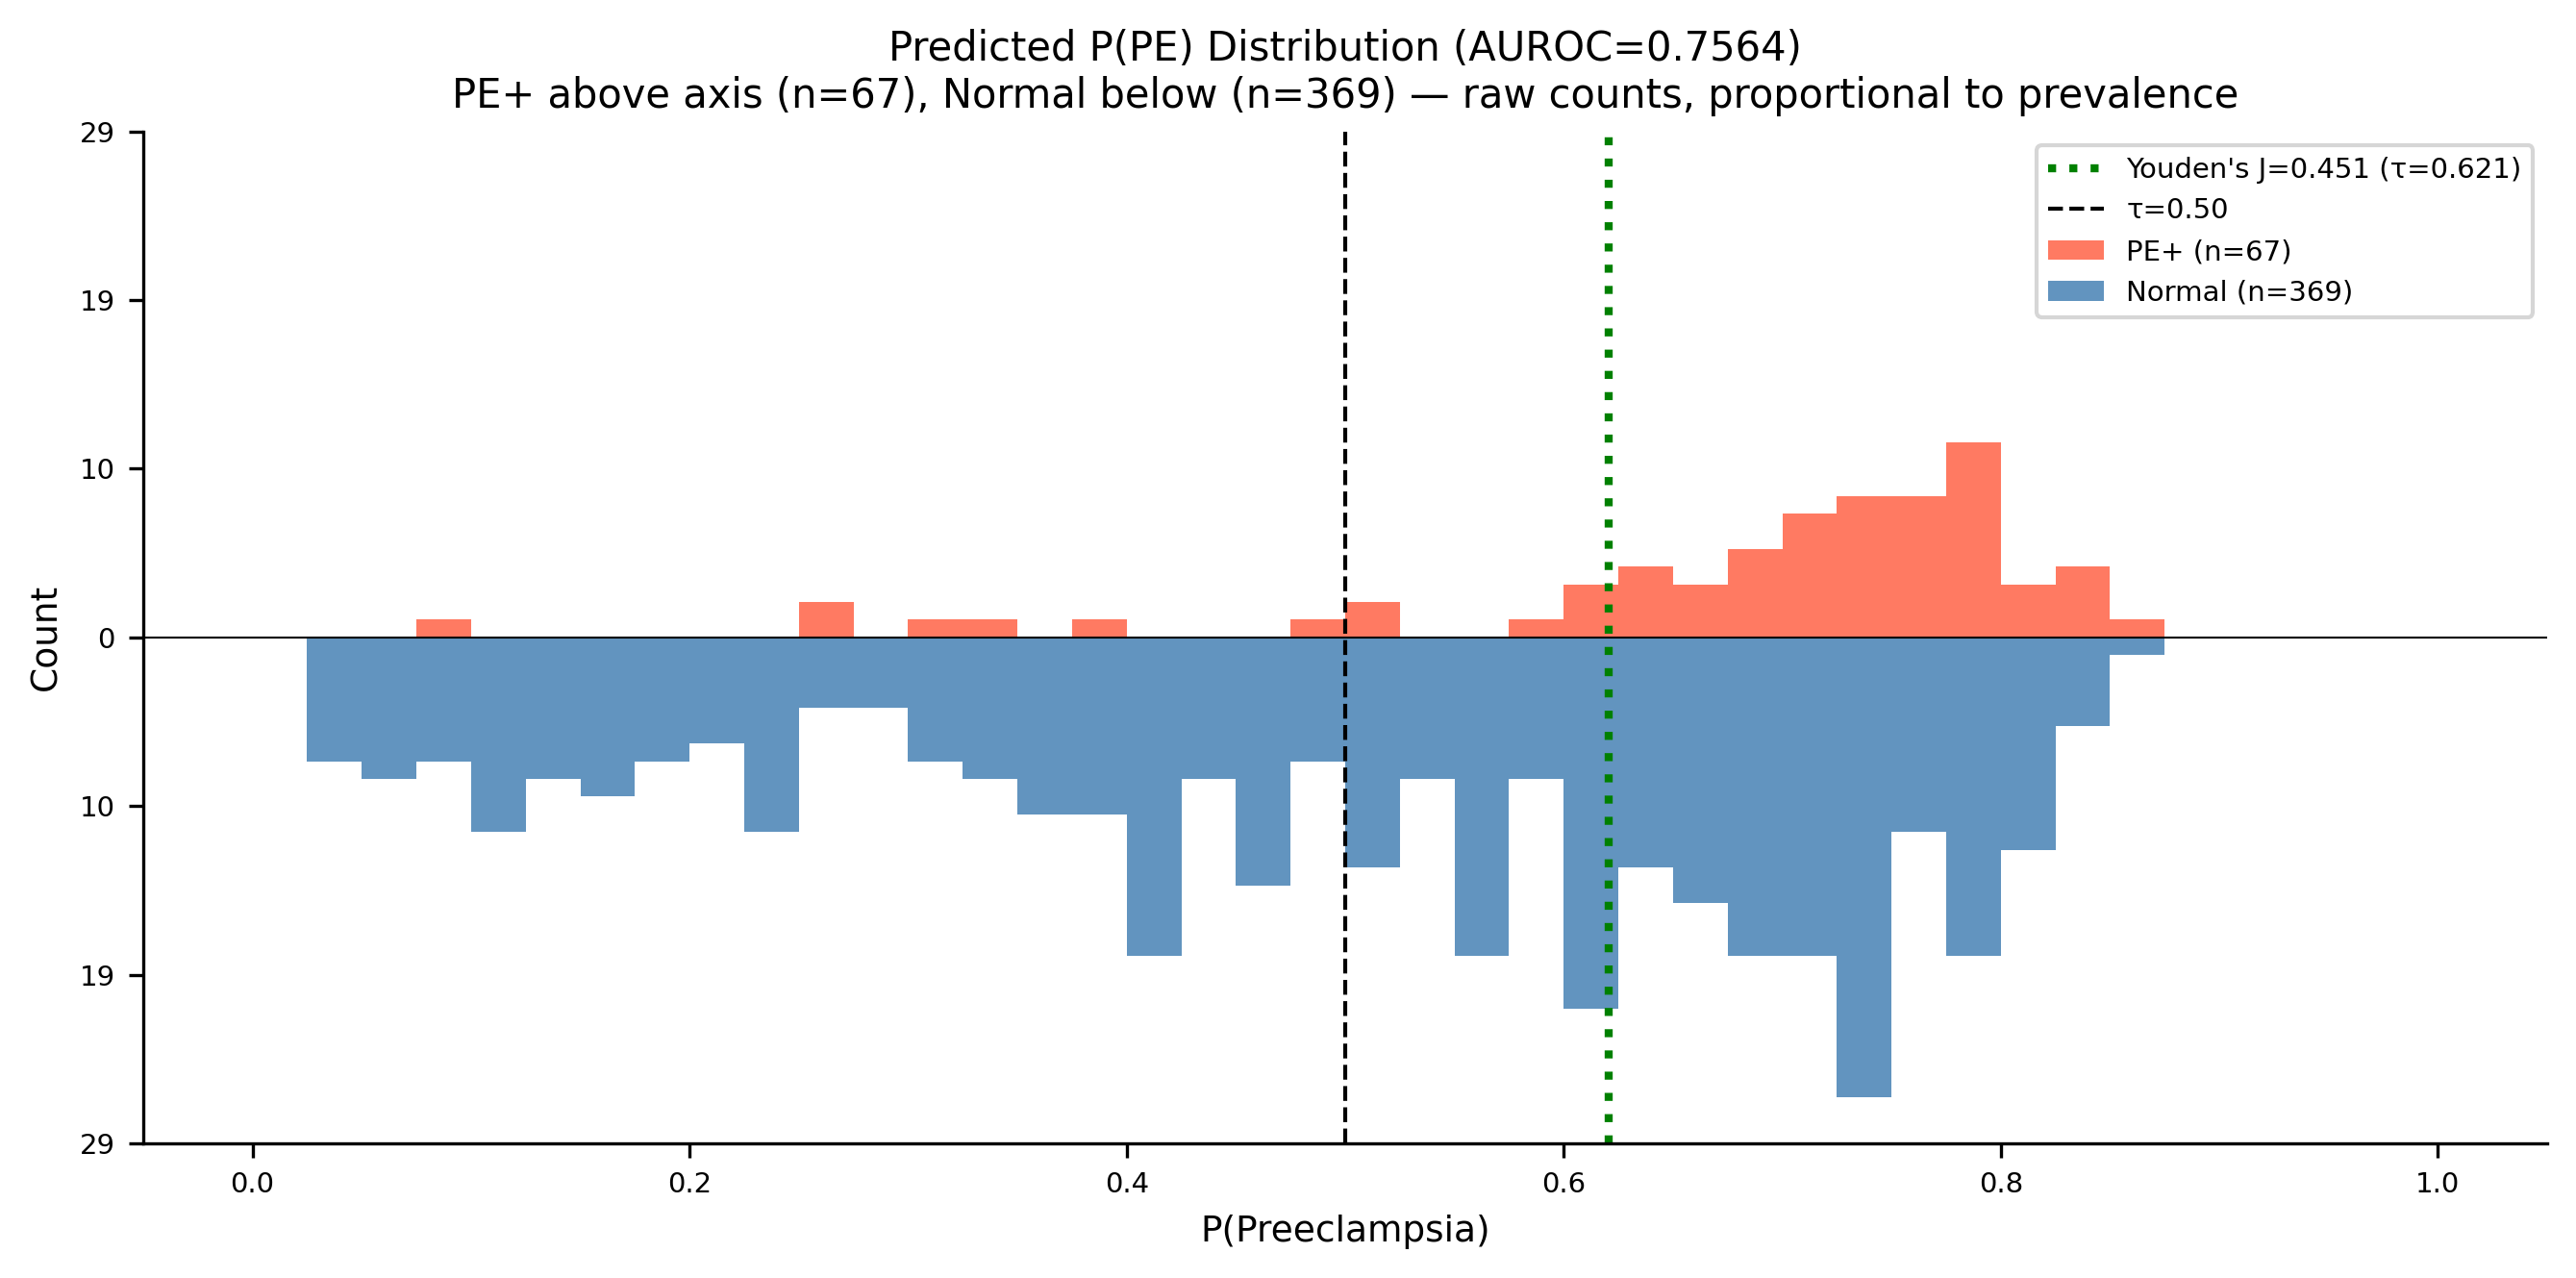
\includegraphics[width=\textwidth]{pred_histogram.png}
    \end{column}
  \end{columns}

  \vspace{0.3em}
  \resizebox{0.45\textwidth}{!}{%
    \begin{tabular}{lc}
      \toprule
      \textbf{Metric} & \textbf{5-Bag Ensemble (Seed 45)} \\
      \midrule
      AUROC & 0.787 \\
      AUPRC & 0.362 \\
      Brier Score & 0.275 \\
      Sensitivity @ 80\% Specificity & 0.582 \\
      \bottomrule
    \end{tabular}
  }%

  \vspace{0.3em}
  \begin{itemize}\usebeamerfont{footline}\color{coolgray}
    \setlength{\itemsep}{1pt}\setlength{\parskip}{0pt}
    \item Best seed out of 20 patient-grouped holdout splits, each with a 5-model bagged ensemble
    \item At 80\% specificity, the model catches \textbf{58\% of PE+ cases} --- reflecting the difficulty of the task under heavy class imbalance ($n=67$ PE vs $n=369$ Normal)
    \item As a \textbf{screening tool}, high sensitivity is preferred --- a false positive triggers further workup, but a missed PE case risks maternal/fetal harm
  \end{itemize}
\end{frame}

% ---------- Subsection Slide: Interpretability --- Saliency ----------
\begin{frame}{Neural Network Modeling --- Saliency Maps}
  \centering
  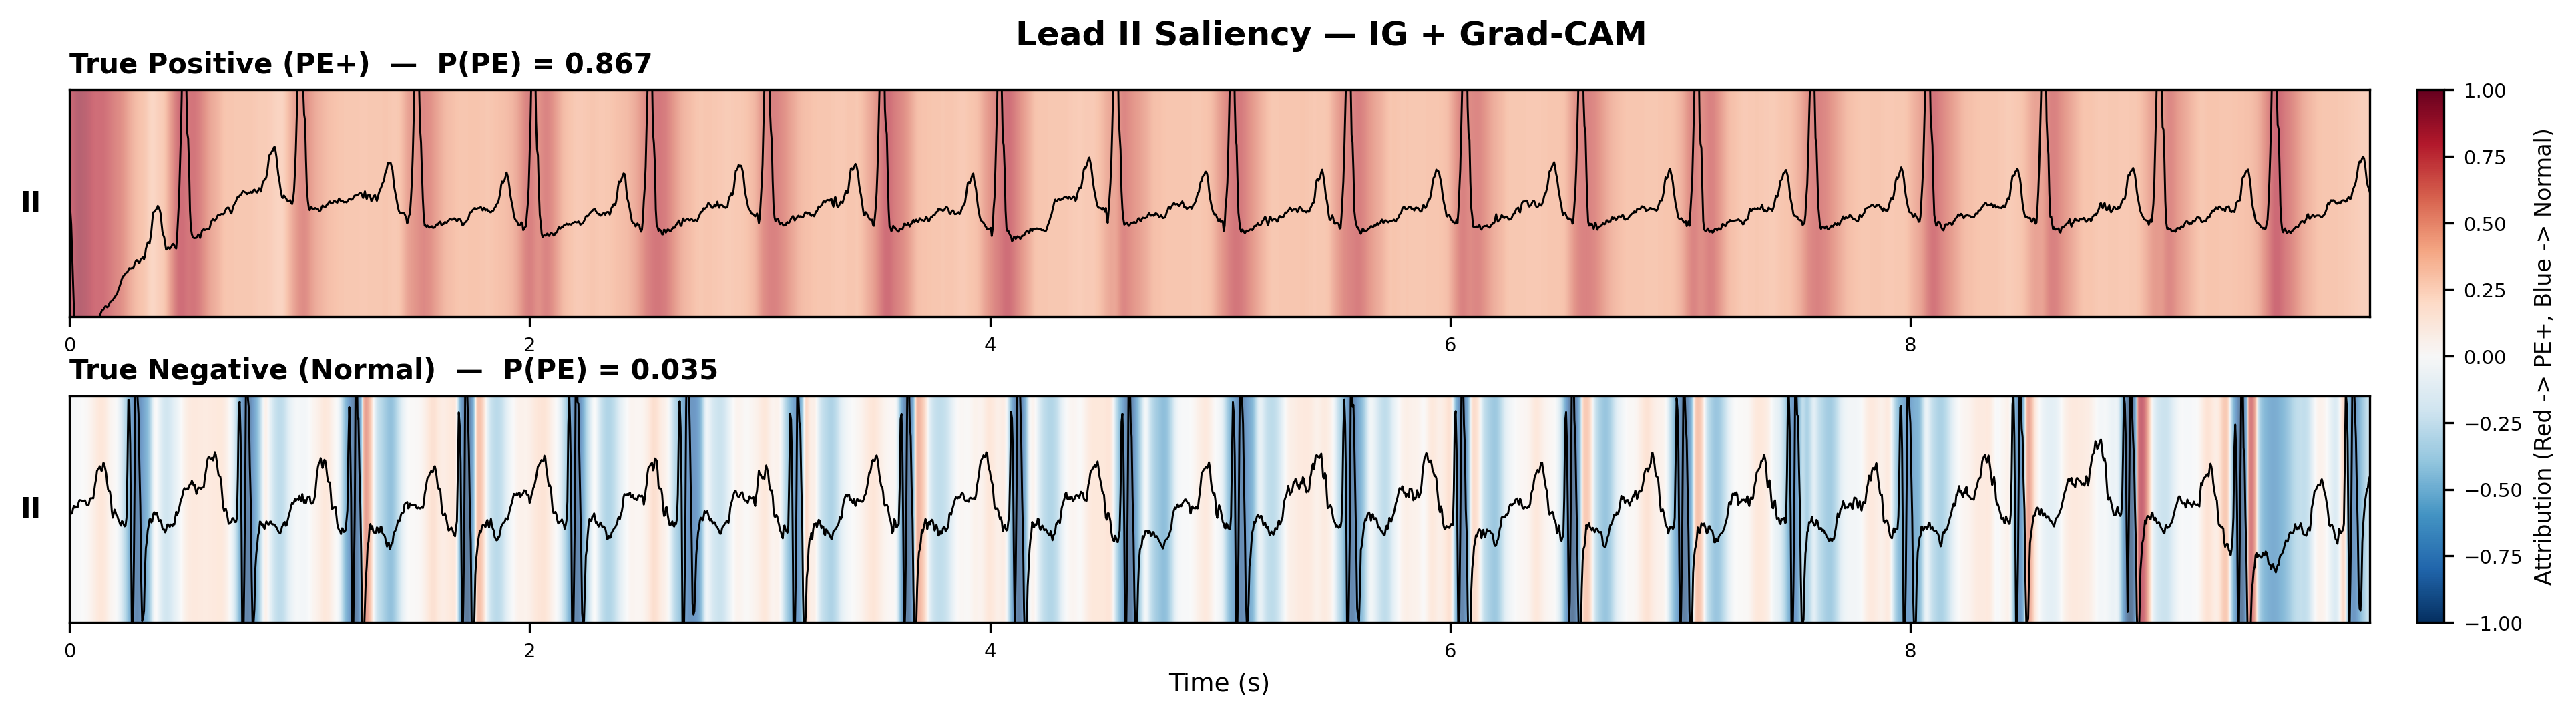
\includegraphics[width=\textwidth]{saliency_poster_lead_II.png}

  \vspace{0.3em}
  \begin{itemize}\usebeamerfont{footline}\color{coolgray}
    \setlength{\itemsep}{1pt}\setlength{\parskip}{0pt}
    \item \textbf{Method:} gradient of PE+ logit w.r.t.\ each sample point --- color intensity $\propto$ regions the model relies on most
    \item Saliency peaks align with \textbf{P-wave} and \textbf{QT-interval} regions --- intervals that literature links to preeclampsia: prolonged QT ($+$21.7\,ms; Aboshady et al.\ 2025) and altered P-wave duration (Angeli et al.\ 2015; Butler et al.\ 2024)

  \end{itemize}
\end{frame}

% ---------- Conclusion Slide ----------
% --- Isolate the background canvas change using curly braces ---
{
\setbeamertemplate{background canvas}{
  
\includegraphics[width=\paperwidth, height=\paperheight]{Conclusion.png}
}
\begin{frame}[plain] % [plain] removes headers, footers, and sidebars for a true full-screen image
  % Leave the frame entirely empty so nothing prints over your image
\end{frame}
}

% ---------- Future Work Slide ----------
\begin{frame}{Future Work}
  \begin{columns}[T]

    % --- Left Column: Narrower to force the column boundary to the left ---
    \begin{column}{0.38\textwidth}
      \color{coolgray} % Removed footline font override to allow normal, larger text size
      
      % Section Header bumped from \small to \large
      {\large\Raleway\bfseries\color{black} Data \& Validation}\\[0.6em]
      \begin{itemize}
        \setlength{\itemsep}{0.4em}
        \item Larger, multi-site datasets
        \item Temporal analysis
        \item Subgroup analysis
      \end{itemize}

      \vspace{1.5em} % Slightly adjusted to balance the larger text

      % Section Header bumped from \small to \large
      {\large\Raleway\bfseries\color{black} Modeling \& Deployment}\\[0.6em]
      \begin{itemize}
        \setlength{\itemsep}{0.4em}
        \item Hybrid ensemble
        \item Clinical decisions support
        \item Lightweight deployment and decreased number of leads
      \end{itemize}
    \end{column}

    % --- Right Column: Expanded and padded on the right to sit closer to the text ---
    \begin{column}{0.58\textwidth}
      \raggedright 

      % Top Section: Callout text and thermometer image
      \begin{minipage}[c]{0.60\textwidth}
        \raggedright
        % Font bumped from \scriptsize to \small for better readability
        \small\Lato\color{black}\bfseries
        End Goal: Make ECG-related diagnoses as easy and available to people as a thermometer is!
      \end{minipage}
      \hfill
      \begin{minipage}[c]{0.36\textwidth}
        \centering
        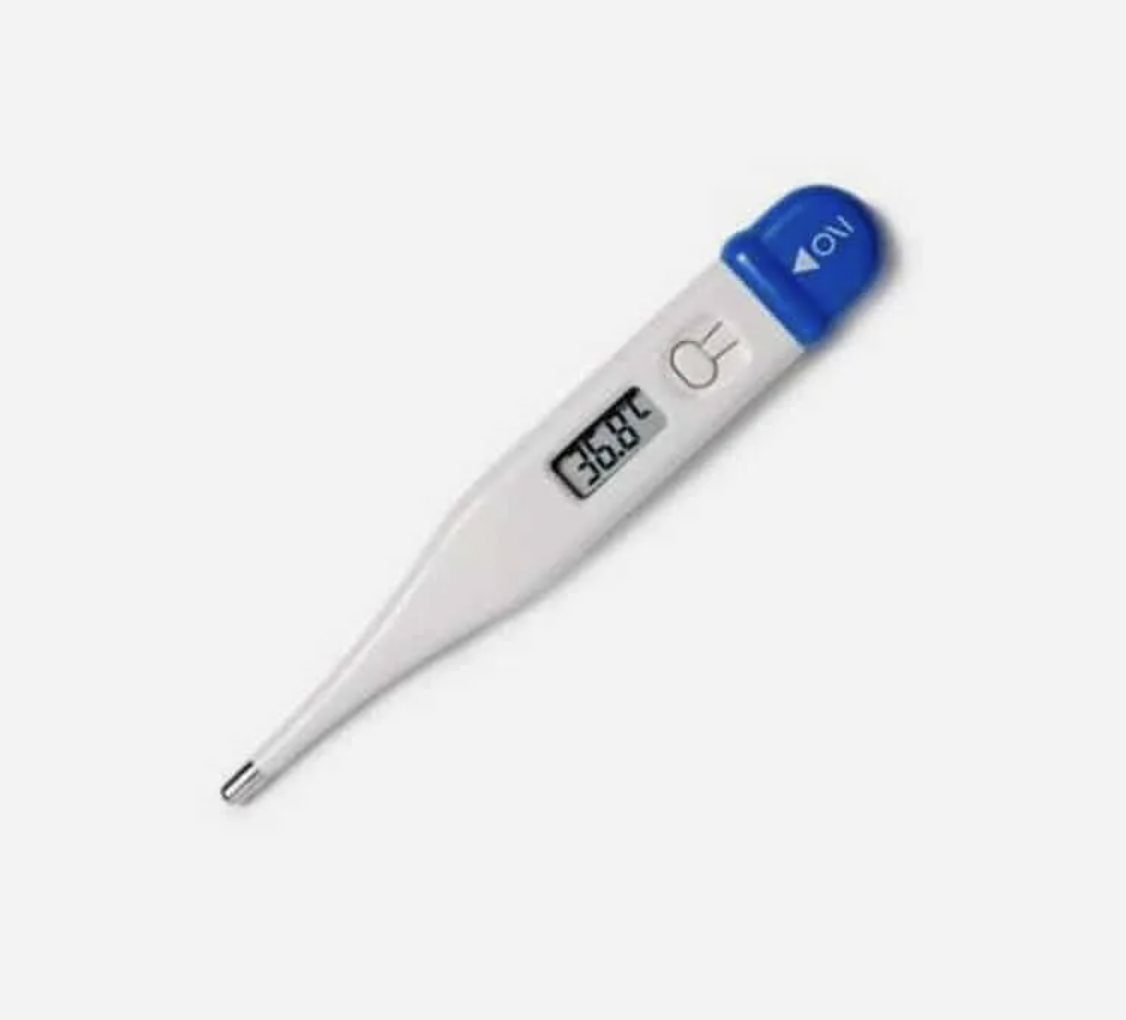
\includegraphics[width=\textwidth]{thermometer.png}
      \end{minipage}

      \vspace{1.0em}

      % Bottom Section: Bedside ECG machine print graphic
      \begin{block}{}
        \label{fig:ecg_print}
        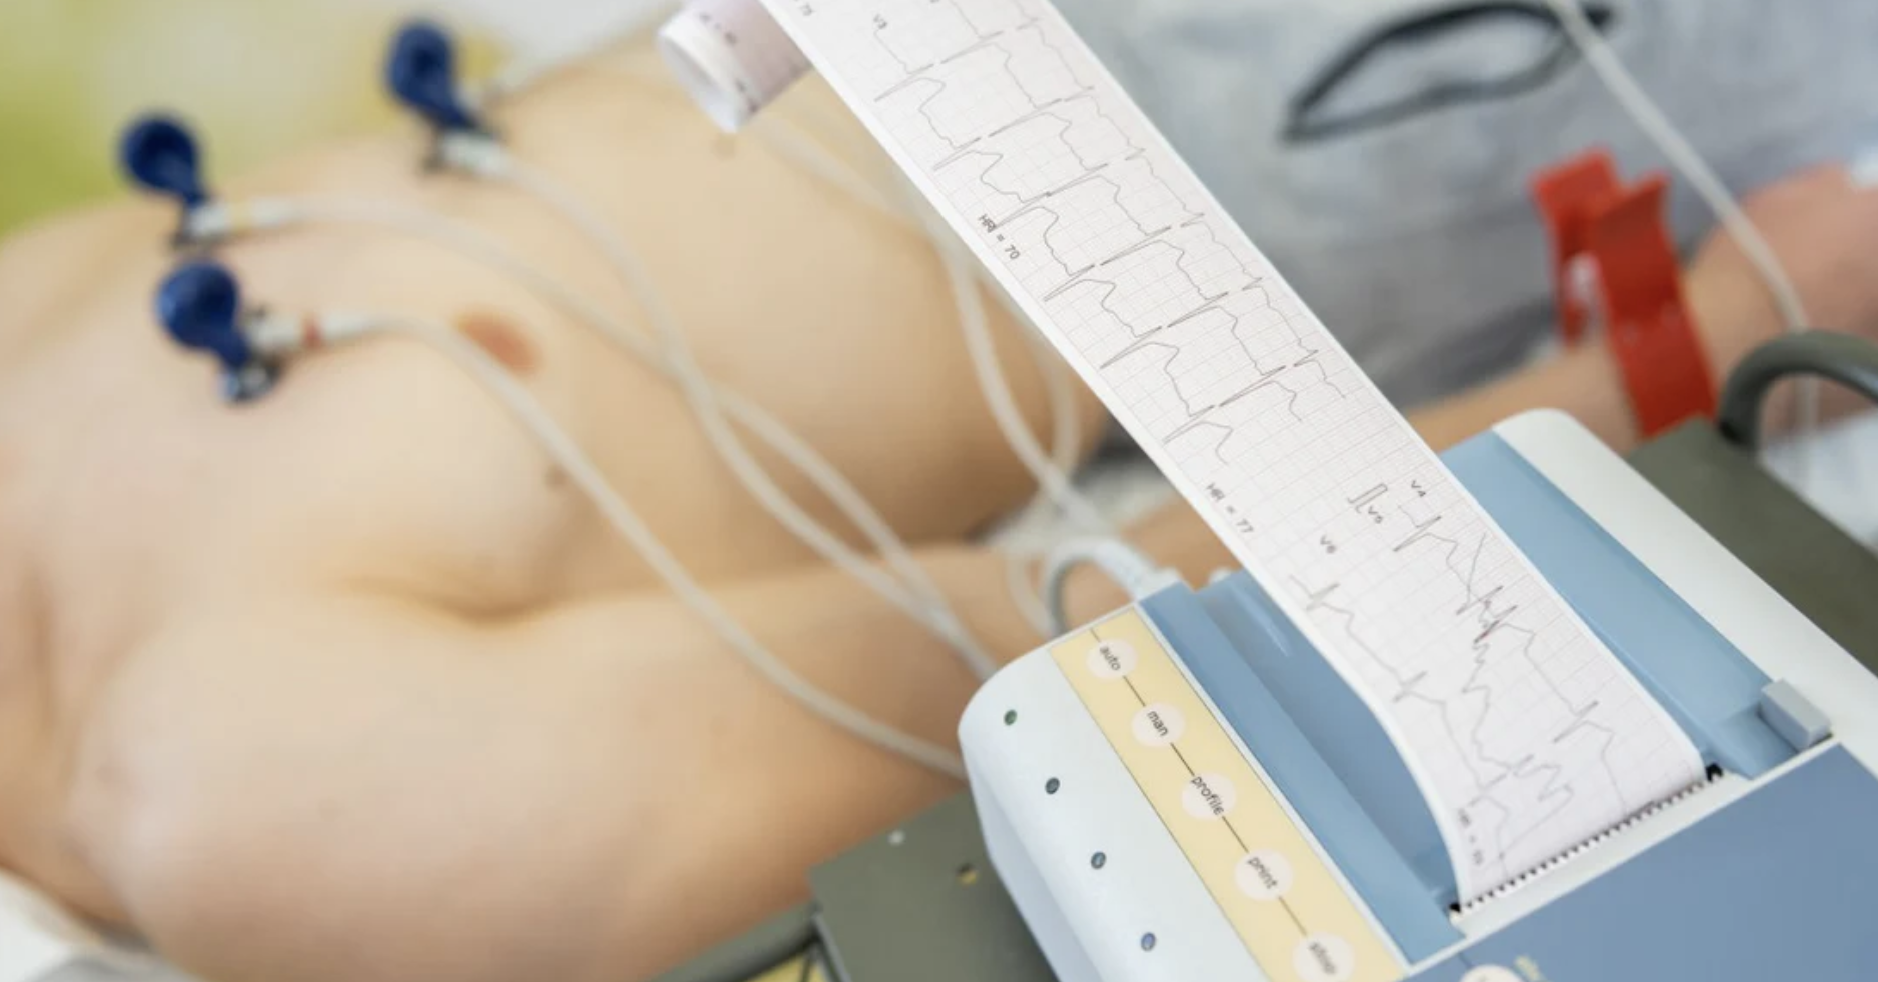
\includegraphics[width=0.95\textwidth]{ecg_printing.png}
      \end{block}
      
      \hfill 
    \end{column}

  \end{columns}
\end{frame}

% ---------- Closing Slide ----------
{%
  \setbeamertemplate{footline}{}%
  \begin{frame}[plain,noframenumbering]
    \begin{tikzpicture}[remember picture,overlay]
      \fill[aggieblue] (current page.south west) rectangle (current page.north east);
    \end{tikzpicture}
    \vfill
    \centering
    {\Raleway\bfseries\Huge\color{white} Thank you}\\[0.6em]
    {\color{aggiegold}\rule{4cm}{0.06cm}}\\[0.8em]
    {\Lato\large\color{white} Questions?}
    \vfill
  \end{frame}
}

\end{document}